\documentclass[french]{report}
\usepackage[utf8]{inputenc}
\usepackage[T1]{fontenc}
\usepackage{fourier}
\usepackage{babel}
\usepackage{graphicx}
\usepackage[x11names, table]{xcolor}
\usepackage{float}
\usepackage{csquotes}
\usepackage{array}
\usepackage{multirow}
\usepackage{biblatex}
\usepackage{svg}
\usepackage[a4paper, portrait, margin=3.5cm]{geometry}
\usepackage{capt-of,booktabs}
\usepackage{pdflscape}

\addbibresource{Biblio.bib}

\newcommand\rmq[1]{\textcolor{red}{\tt #1}}

\title{Mémoire Master}
\author{faycalchefai1 }
\date{September 2021}

\begin{document}
%Page de garde


\begin{titlepage}
\begin{center}
    \large{République Algérienne Démocratique et Populaire}\\
    \large{Ministère de l'Enseignement Supérieur et de la Recherche Scientifique}\\
    \large{Université A. Mira de Bejaia}\\
    \large{Faculté des Sciences Exactes}\\
    \large{Département d'Informatique}\\

    \begin{figure}[h!]
    \centering
    
\includegraphics[width=6cm]{images/logo1.jpg}
    \end{figure}
	
    \LARGE{\textbf{Mémoire de Fin de Cycle}} \\[2ex]
     En vue de l'obtention du diplôme de Master en Informatique \\[1ex]
    
    \textit{\textbf{Thème}}\\[1ex]
	\rule{11,5cm}{1pt}
    {\LARGE{\textbf{{\\Conception et réalisation d'une application Web d'offres
    de services professionnels \\}}}}
	\rule{11,5cm}{1pt}\\
	\vspace{0.2cm}
\end{center}

\begin{center}
    \large Réalisé par

    \paragraph{}

    \begin{tabular}{l l l l}	
        M. CHEFAI Fayçal & & & M. BORDJIHANE Sami \\
    \end{tabular}

    \large Devant le jury composé de
\end{center}
\paragraph{}

\begin{table}[h!]
    \centering
    \begin{tabular}{l l l }
     & Promotion 2020 - 2021 &	\\
    \end{tabular}    
\end{table}
\end{titlepage}

%Fin de page de garde

\tableofcontents
\listoffigures
\listoftables


%Début introduction
\chapter*{Introduction Générale}
Depuis sa naissance, l’humain n’a cessé d’évoluer et de chercher le moyen de rendre sa vie plus confortable.
L’internet fut une étape crucial de se développement.

C’est en 1973 que le concept d’Internet a vu le jour, et jusqu’à aujourd’hui, elle n’a cessé d’évoluer
et de proposer de nouvelles technologies pour améliorer le quotidien des gens,

Le chercheur britannique Tim Berners-Lee a inventé le World Wide Web en 1989. À l’origine, le projet a 
été conçu et développé pour que des scientifiques travaillant dans des universités et instituts du monde
entier puissent s'échanger des informations instantanément. L'idée de base du WWW était de combiner les 
technologies des ordinateurs personnels, des réseaux informatiques et de l'hypertexte pour créer un système
d'information mondial, puissant et facile à utiliser.
		

Aujourd’hui le WEB occupe une grande place dans notre vie, que se soit notre vie personnelle ou professionnelle.
La majorité des activité quotidiennes nécessite un accès directe et rapide au réseaux, par exemple un chef de projet
qui doit gérer son équipe et son projet à distance, ou bien une personne qui voudrait faire ses courses, 
sans se déplacer à l’aide de sites marchands.

Parmi les types d’applications disponibles, on trouve les applications web. Celles ci sont des sites web se comportent
comme de véritables applications pour ordinateur ou téléphone. La plus part des entreprises se concentrent 
sur le développement de se genre d’application car elles sont avantageuse niveau accessibilité.
En effet elle offre une grande mobilité et un accès facile à partir de n’importe quel appareil mobile,
n’importe où et à tout moment avec une simple connexion Internet.

Notre choix de développer une application web se justifie par le fait qu'elle est un moyen très utile
et efficace pour exposer et offrir des services via Internet grâce à l'accessibilité qu'elle offre
aux utilisateurs ou bien aux clients indépendamment de leurs emplacements physiques, ce qui nous 
permettra de rapprocher les fournisseurs des clients.

Notre projet vise à simplifier le processus que rencontre la plus part des gens lors de la recherche
d’une personne qualifiée dans un domaine, c’est à dire la recherche de gens fiables, de préférence
qui habitent dans une région alentour, qui a une certaine expérience et qu’on pourra contacter sans problème.

Dans ce présent rapport, nous présenterons les différentes étapes que nous avons suivies lors du
développement de notre application web. Notamment, la démarche suivie, les diagrammes conçus,
ainsi que les différents langages et outils utilisés. Enfin, nous clôturerons ce travail avec 
une conclusion générale et quelques perspectives qui permettront d'améliorer notre solution.

%Fin introduction


%Début du chapitre 1
\chapter{Étude Préalable}

\section{Introduction}
Dans ce chapitre, nous évoquerons la problématique au centre de notre application.
Nous ferons référence à quelques détails de cette problématique et nous proposerons
une solution informatique sous forme d’application web. Pour clore ce chapitre,
nous parlerons du langage de modélisation utilisé au cours de notre conception. 

\section{Identification de la problématique}
Le problème que rencontre beaucoup de gens dans leur vie quotidienne est la recherche
de professionnels compétents ainsi que des informations sur leurs professions, parmi elles on retrouve : 

	\begin{itemize}
	    \item Contacts du professionnel;
	    \item Informations sur les tarifs;
	    \item Disponibilité; 
	    \item Travaux antérieurs;
	    \item Fiabilité. 
	\end{itemize}

La méthode classique est la recherche manuelle, on peut appeler ça "Du bouche à oreille".
Les informations sur les personnes recherchées peuvent ne pas être correctes, ou du moins pas fiables. 

Prenons un exemple, soit disant que vous avez une panne d'électricité à la maison, vous faites quoi?
Appeler un électricien est le premier réflexe pour les non bricoleurs. Le fait de chercher
un numéro de téléphone, de s'assurer que la personne est compétente, de voir les tarifs de la personne
à l'avance peut prendre du temps, et souvent on est déçus du résultat.

Le but est de minimiser le temps passé sur les recherches et d'augmenter le taux de satisfaction chez 
les clients. Pour cela nous avons décidé de réaliser cette application.

\section{Présentation de la solution proposée}
Pour remédier à la problématique identifiée ci-dessus, nous proposons une solution informatique sous
forme d'application web fournissant les fonctionnalités suivantes :

\begin{itemize}
	\item Recherche filtrée des services (selon le tarif, le domaine, le lieu, etc.);
	\item Accès aux informations liées au service (tarifs, durée de réalisation, etc.);
	\item Possibilité de contacter le fournisseur du service;
	\item Possibilité de commander un service; 
	\item Possibilité de suivi de ses commandes;
	\item Mise en place d'un système de notation des services;
	\item Ajout de nouveaux services;
	\item Édition et suppression des services.
\end{itemize}

\section{Besoins fonctionnels}
\begin{itemize}
	\item Le système permettra aux clients et fournisseurs de communiquer.
	\item Le système permettra aux clients de chercher, consulter et commander un service.
	\item Le système permettra aux clients d'ajouter un avis;.
	\item Le système permettra aux fournisseurs d'ajouter, modifier ou supprimer un service.
	\item Le système permettra d'afficher quelques statistiques pour les fournisseurs.
\end{itemize}

\section{Besoins non fonctionnels}
\begin{itemize}
	\item Vérifier ou valider l'identité d'une personne ou identifier toute autre entité pour contrôler 
	l'accès à un réseau;
	\item Choisir des solutions adéquates pour protéger l'utilisateur;
	\item Capacité du site à aider à la réalisation de l'activité d'utilisateur pour laquelle il a été conçu;
	\item Capacité du site à être opérationnel à tout instant.
\end{itemize}

\section{Langage de modélisation}
    \subsection{Unified Model Language}
    Dans la carrière d'un développeur, il sera confronté à concevoir et réaliser des applications
    très complexes en tout genre. L'UML aide à gérer cette complexité pour que au cours de la réalisation,
    le développeur ne dévie pas de l'objectif final, c'est à dire satisfaire le client. \cite{learningUML}
    
    Les systèmes développés ont pour but de satisfaire des objectifs précis formulés par le client.
    Ce client donc fait partie du processus de développement. Ils imaginent, décrivent à quoi peut
    ressembler le système final. Le rôle du développeur est de bien capturer les besoins du client à
    travers la modélisation.\cite{unhelkar2017software}
    
    \begin{figure}[H]
        \centering
        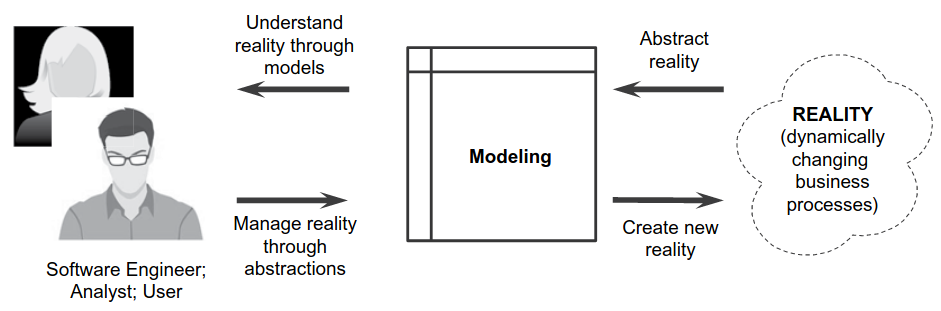
\includegraphics[width=1\textwidth]{images/modelisation.png}
        \caption{Importance de la modélisation en génie logiciel}
        \label{Importance de la modélisation}
    \end{figure}

        \subsubsection{Définition}
        UML est un acronyme en Anglais \emph{"Unified Modeling Langage"}, en français ça donne 
	\emph{"Langage de modélisation unifié"}. C'est donc un langage de modélisation ou bien
	un langage visuel, car il utilise un ensemble de diagrammes pour décrire la structure 
	et le comportement du système.\cite{geeksforgeeks}
        
        L'UML a était standardisé en 1997 par l'OMG (Object Management Group). L'organisation
	internationale de normalisation (ISO) a publié UML en tant que norme approuvée en 2005.
	UML a été révisé au fil des ans et est revu périodiquement.\cite{geeksforgeeks}
        
        \begin{figure}[!h] 
        \center 
            
\includegraphics[width=0.3\textwidth,keepaspectratio]{images/uml-logo-large.jpg} 
            \caption{Logo de UML.}
            \label{UML logo}
        \end{figure}
        
        \subsubsection{Pourquoi utiliser UML?}
        \begin{description}
            \item[UML est un langage de modélisation standard] c'est a dire 
            qu'il est indépendant du langage de programmation. \cite{IBM}
            \item[UML est un langage et non une méthodologie], 
	    il peut facilement s'intégrer dans la manière de travail des entreprises sans nécessiter de changement.\cite{IBM}
            \item[UML fournis des diagrammes] 
	    qui facilitent la compréhension d'une application en développement.
	    Cela permettra aux personnes maîtrisant UML de rejoindre plus facilement
	    votre projet et de devenir rapidement productifs.\cite{IBM}
        \end{description}
        
        \subsubsection{Les diagrammes}
        UML propose 14 diagrammes en tout. Les diagrammes standards les plus utiles sont :
	diagramme de cas d'utilisation, diagramme de classes, diagramme de séquence.
            \begin{description}
                \item[Diagramme de cas d'utilisation :]
                Un cas d'utilisation illustre une unité de fonctionnalité fournie par le système.
		L'objectif principal du diagramme de cas d'utilisation est d'aider les équipes de développement
		à visualiser les exigences fonctionnelles d'un système, y compris la relation des « acteurs »
		(êtres humains qui interagiront avec le système) avec les processus essentiels,
		ainsi que les relations entre les différents cas d'utilisation.\cite{IBM}
                
                Pour afficher un cas d'utilisation sur un diagramme de cas d'utilisation, 
		vous dessinez un ovale au milieu du diagramme et placez le nom du cas d'utilisation au centre.\cite{IBM}
                
                Pour dessiner un acteur (indiquant un utilisateur du système) sur un diagramme de cas d'utilisation,
		vous dessinez une personne bâton à gauche ou à droite de votre diagramme.\cite{IBM}
                
                Des lignes simples sont utilisées pour décrire les relations entre les acteurs et les cas d'utilisation,
		comme le montre la figure.\cite{IBM}
                
                \begin{figure}[!h] 
                    \center 
                    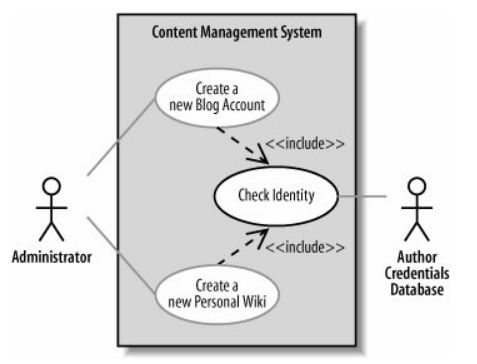
\includegraphics[width=0.7\textwidth,keepaspectratio]{images/use case exemple.png} 
                    \caption{Exemple de diagramme de cas d'utilisation}
                    \label{UML logo}
                \end{figure}
                
                \item[Diagramme de classe :]
                Le diagramme de classes montre comment les différentes entités (personnes, choses et données)
		sont liées les unes aux autres ; en d'autres termes, il montre les structures statiques du système.\cite{IBM}
                
                Une classe est représentée sur le diagramme de classe sous la forme d'un rectangle avec trois sections
		horizontales; la section du milieu contient les attributs de la classe ;
		et la section inférieure contient les opérations de la classe (ou « méthodes »). \cite{IBM}
                \begin{figure}[!h] 
                    \center 
                    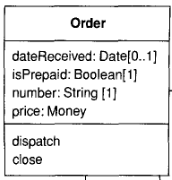
\includegraphics[width=0.2\textwidth,keepaspectratio]{images/class example.png} 
                    \caption{Exemple d'une classe}
                    \label{UML logo}
                \end{figure}
                
                Les classes sont liées entre elles grâce à différents type de relations
                \begin{figure}[!h] 
                    \center 
                    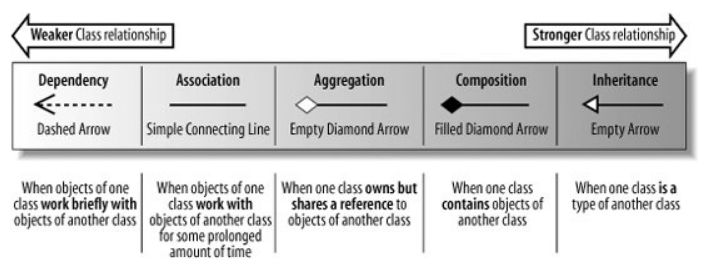
\includegraphics[width=0.8\textwidth,keepaspectratio]{images/diag class relation exemple.png} 
                    \caption{Les types de relations}
                    \label{UML logo}
                \end{figure}
                
                Une relation d'association entre deux classes peut également véhiculer des informations 
		sur le nombre de comptes d'objets (instances) à chaque extrémité de l'association.
		Ce nombre d'objets est appelé multiplicité. Les multiplicités indiquent le nombre d'objets
		d'une classe liés à un objet d'une autre classe.\cite{IBM}
                
                \begin{figure}[H] 
                    \center 
                    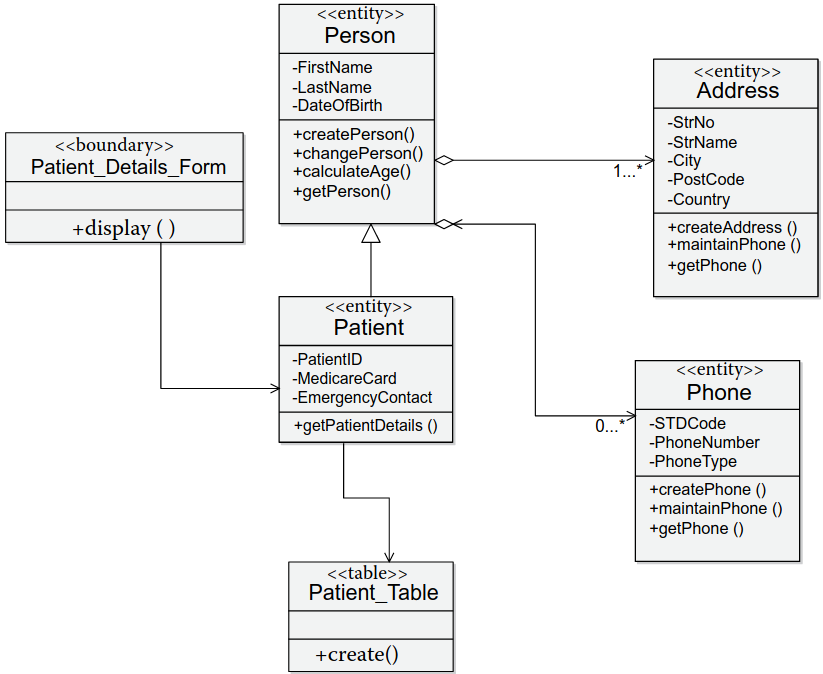
\includegraphics[width=0.7\textwidth,keepaspectratio]{images/diag classe example.png} 
                    \caption{Exemple d'un diagramme de classe}
                    \label{UML logo}
                \end{figure}
                
                \item[Diagramme de séquence :]
                Uml propose des diagrammes d'interaction, qui décrivent comment des groupes d'objets 
		collaborent dans certains comportements. Le plus courant est le diagramme de séquence.\cite{fowler2004uml}
                
                En règle générale, un diagramme de séquence capture le comportement d'un seul scénario. 
		Le diagramme montre un certain nombre d'exemples d'objets et les messages qui sont transmis 
		entre ces objets dans le cas d'utilisation.\cite{fowler2004uml}
                
                Un diagramme de séquence a deux dimensions : la dimension verticale montre la séquence des
		messages/appels dans l'ordre temporel dans lequel ils se produisent ; 
		la dimension horizontale montre les instances d'objet auxquelles les messages sont envoyés.\cite{IBM}
                
                Le diagramme de séquence utilise un ensemble de notations pour décrire les interactions dans le temps.
                \begin{figure}[H] 
                    \center 
                    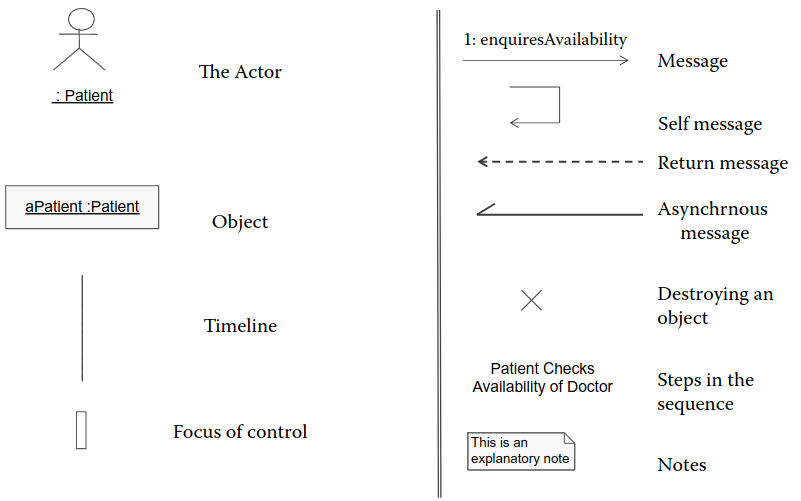
\includegraphics[width=0.7\textwidth,keepaspectratio]{images/diag sequence component.png} 
                    \caption{Les notations du diagramme de séquence}
                    \label{Sequence diag notations}
                \end{figure}
            \end{description}

\section{Conclusion}
L'objectif des systèmes développés est d'automatiser et faciliter des taches, habituellement 
qui demanderais des efforts et du temps.

Le but cherché derrière le développement de notre système est de d'optimiser la recherche
de gens compétents et de remplacer les méthodes manuelles habituelles.

Nous proposons une application web qui mettra en relation deux camps, ceux qui cherchent
des personnes compétentes qui offrent des services et ces personnes là.

Dans ce chapitre, nous avons évoqué un ensemble de difficultés du quotidien sous forme 
de problématique. Nous avons essayé de proposer une solution adéquate.

Dans une partie de ce chapitre, nous avons fait une brève explication du langage de 
modélisation que nous allons utiliser pour la réalisation de cette application, qui est l'UML.

Des explications sur l'utilité d'utiliser un langage de modélisation ont été évoqués ainsi
que les différents principaux diagrammes que nous utiliserons dans les prochaines étapes du développement.


%Fin du chapitre 1



%Début du chapitre 2
\chapter{Analyse et Conception}


\section{Identification des acteurs et leurs rôles }
Dans notre système, on distingue les acteurs suivants :

    \begin{table}[h!]
    \centering
    \begin{tabular}{ |m{3cm}|m{3cm}|m{5.5cm}| }
    \hline
    \textbf{Acteurs} & \textbf{Codification} & \textbf{Rôle} \\
    \hline
    Administrateur & Admin & Gérer le système en effectuant des opérations d'ajout,
    de modification et de suppression sur la base de données \\
    \hline
    Client & Client & Inscription, connexion, consultation de services, contacter des fournisseurs,
    laisser des avis, commander des services, gérer ses commandes \\
    \hline
    Fournisseur & Fournisseur & Inscription, connexion, gestion de services, gestion de la messagerie \\
    \hline
    \end{tabular}
    \caption{Identification des acteurs et leurs rôles.}
    \label{Tableaux:1}
    \end{table}

\section{Identification des cas d'utilisations}
\begin{table}[H]
    \centering
    \begin{tabular}{|m{5cm}|m{5cm}|}
        \hline
         \textbf{Cas d'utilisation} & \textbf{Acteurs} \\
        \hline
        Inscription & \multirow{5}{5cm}{Client, Fournisseur} \\
        Authentification & \\
        Gestion des commandes & \\
        Gestion des avis & \\
        Gestion des messages & \\
        Modification du compte & \\
        \hline
        Consultation de services & \multirow{2}{5cm}{Client} \\
        Recherche de services & \\
        \hline
        Ajout de services & \multirow{3}{5cm}{Fournisseur} \\
        Suppression de services & \\
        Modification de services & \\
        \hline
        Connexion & \multirow{7}{5cm}{Administrateur} \\
        Gestion des clients & \\
        Gestion des fournisseurs & \\
        Gestion des messages & \\
        Gestion des commandes & \\
        Gestion des avis & \\
        Suppression des services & \\
        \hline
    \end{tabular}
    \caption{Identification des cas d'utilisation.}
    \label{tab:my_label}
\end{table}
\newpage
\section{Diagramme de cas d'utilisation}

\begin{itemize}
    \item \underline{Générale :}
        \begin{figure}[H]
            \centering
            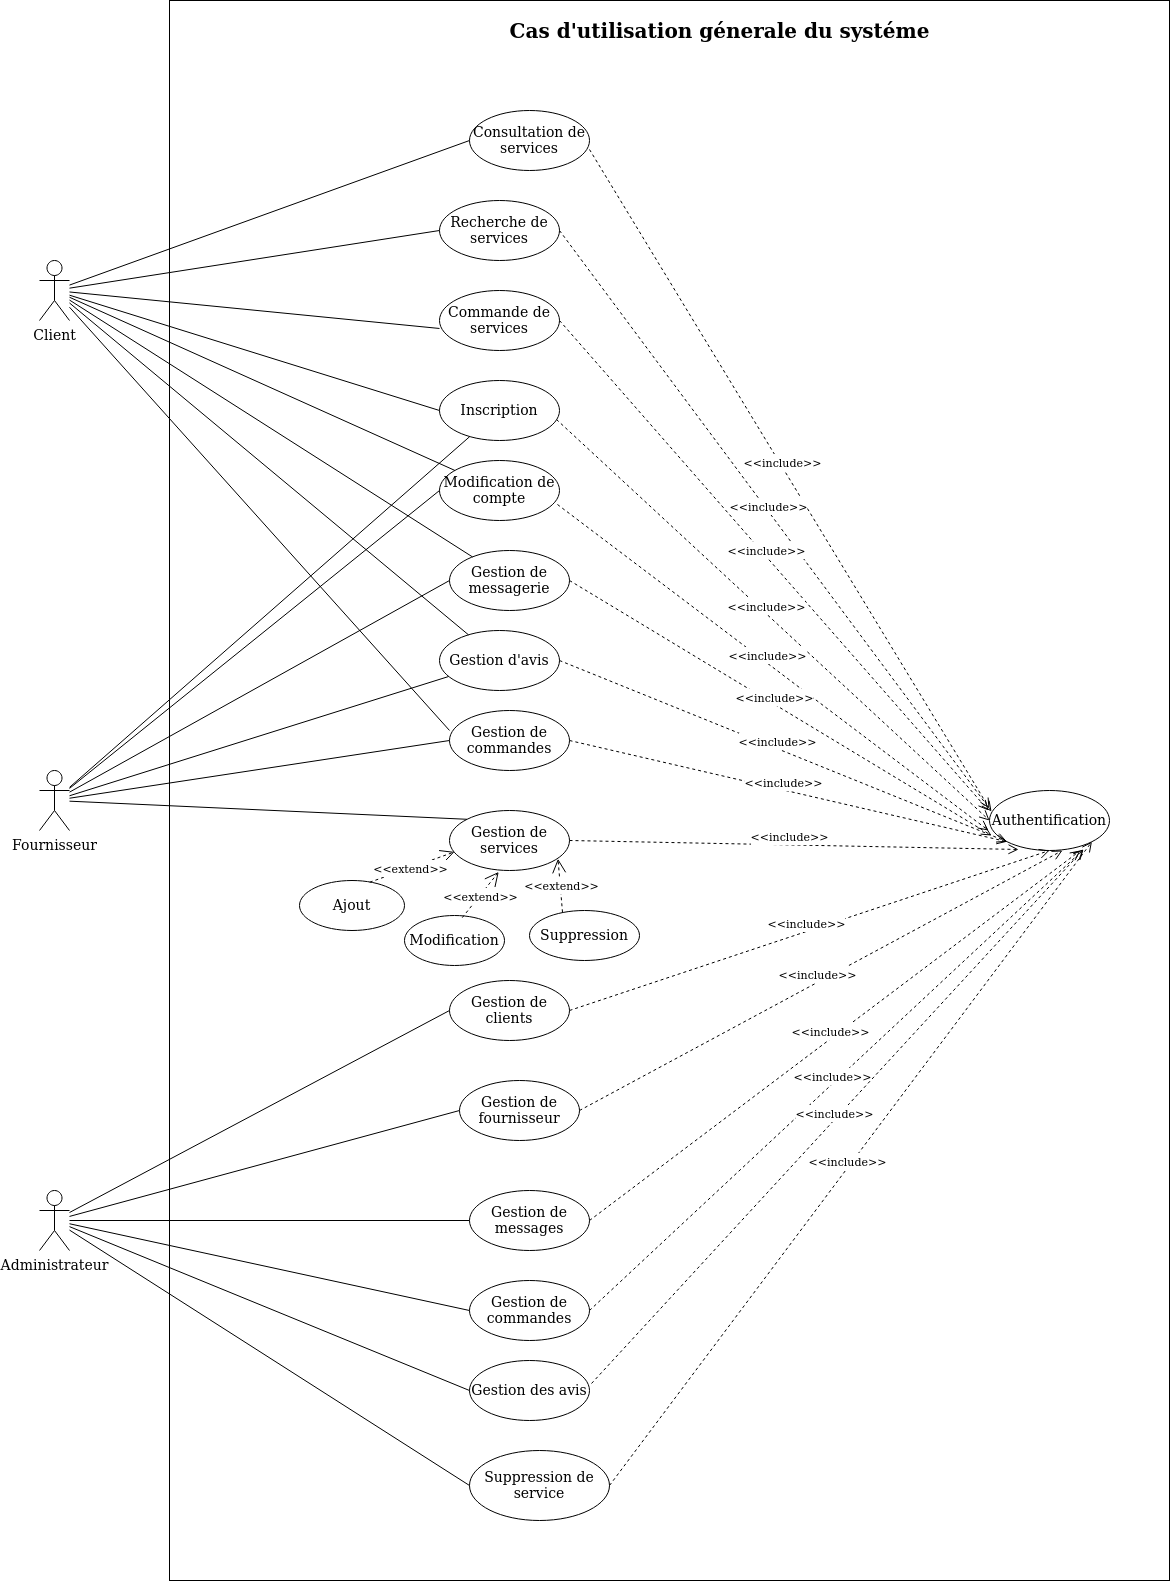
\includegraphics[width=1\textwidth]{images/Use cas general.drawio.png}
            \caption{Diagramme de cas d'utilisation générale}
            \label{Use case diag}
        \end{figure}
        
\newpage
    \item \underline{Client :} 
        \begin{figure}[H]
            \centering
            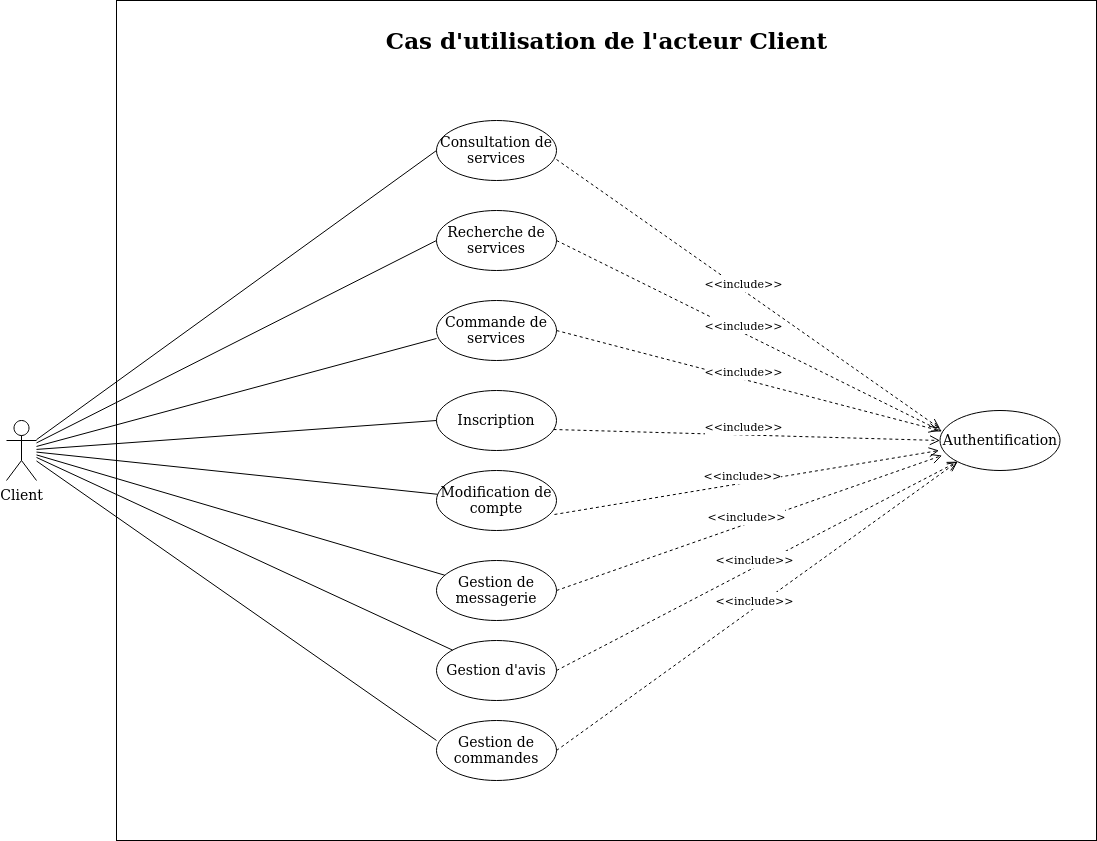
\includegraphics[width=1\textwidth]{images/Use Case Client.drawio.png}
            \caption{Diagramme de cas d'utilisation de l'acteur Client}
            \label{fig:my_label}
        \end{figure}
        
\newpage
    \item \underline{Fournisseur :}
        \begin{figure}[H]
            \centering
            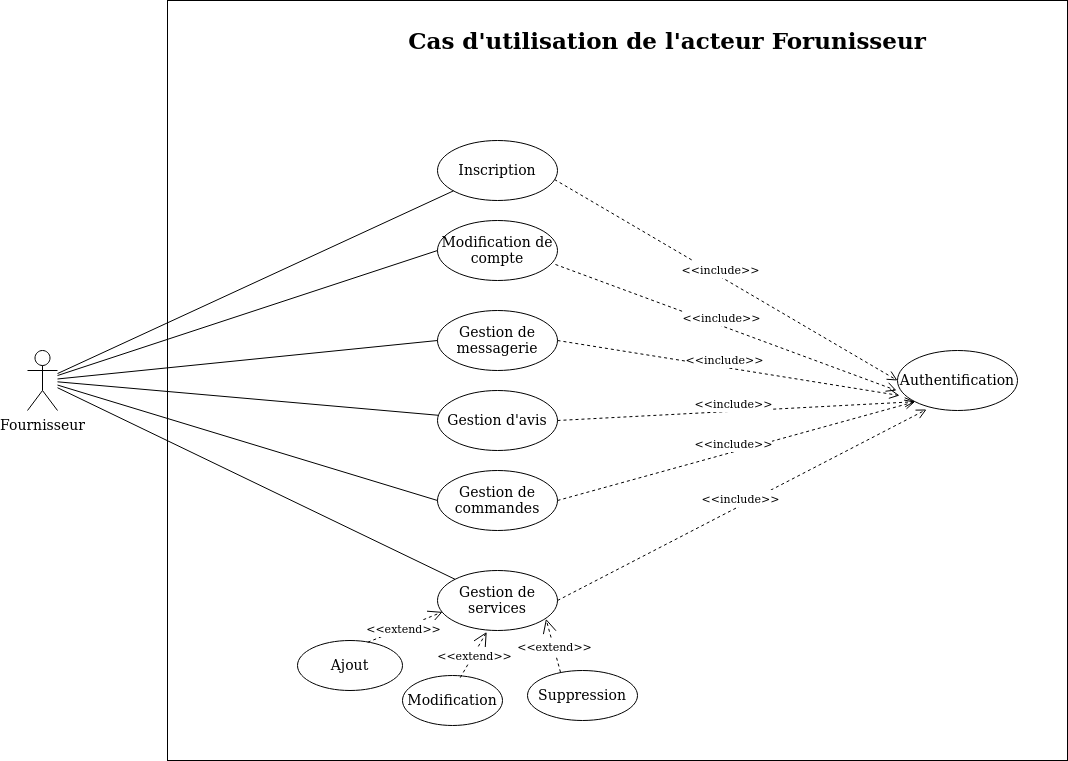
\includegraphics[width=1\textwidth]{images/Use case Fournisseur.drawio.png}
            \caption{Diagramme de cas d'utilisation de l'acteur Fournisseur}
            \label{fig:my_label}
        \end{figure}
        
\newpage
    \item \underline{Administrateur :}
        \begin{figure}[H]
            \centering
            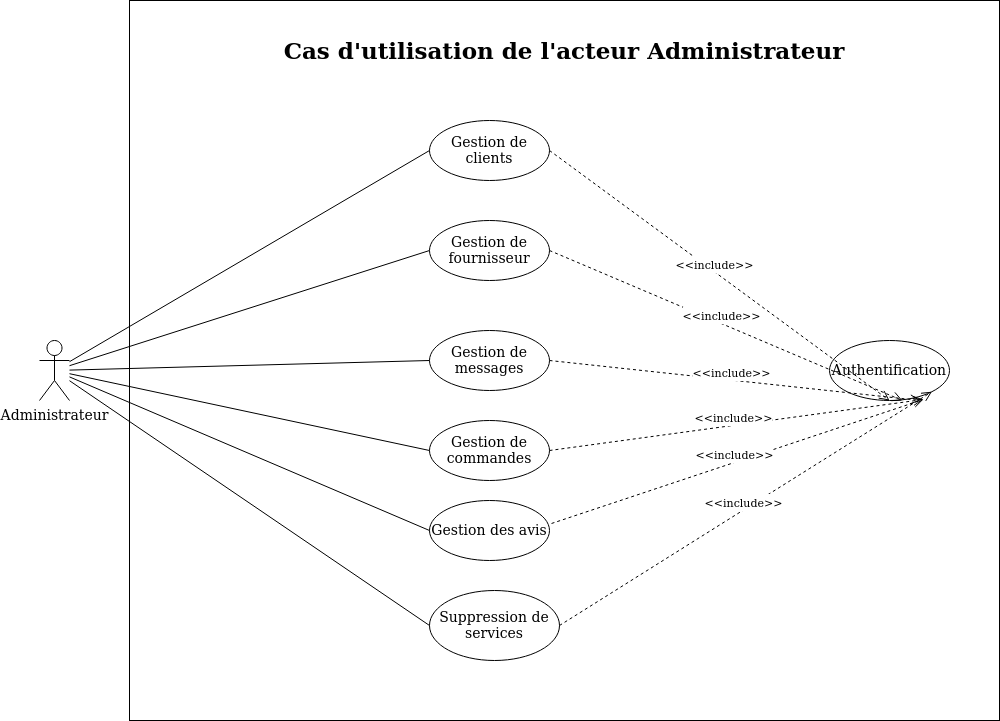
\includegraphics[width=1\textwidth]{images/Use case Administrateur.drawio.png}
            \caption{Diagramme de cas d'utilisation de l'acteur Administrateur}
            \label{fig:my_label}
        \end{figure}
\end{itemize}

\section{Description textuel des cas d'utilisation}
    La description textuel d’un cas d’utilisation permet de :
    
    \begin{itemize}
        \item Clarifier le déroulement de la fonctionnalité 
        \item Décrire la chronologie des actions qui devront être réalisées 
        \item D’identifier les parties redondantes pour en déduire de cas d’utilisations
plus précises qui seront utilisées par inclusion, extension ou généralisation 
        \item D’indiquer d’éventuelles contraintes déjà connues et dont les développeurs
vont devoir tenir compte lors de la réalisation du l’application, aussi les
descriptions peuvent aider à découvrir d’autres cas d’utilisations que l’on
pourrait ajouter. 
    \end{itemize}
    
\newpage
    \begin{description} 
        \item[Inscription] \hfill \\
        \begin{minipage}{\linewidth}
        \centering
            \def\arraystretch{2}
            \begin{tabular}{|m{3cm}|m{9cm}|}
                \hline
                Titre                & Inscription  \\ 
                \hline
                Résumé               & L'inscription permet aux utilisateurs de s'inscrire pour pouvoir accéder 
		au fonctionnalités de l'application \\ 
                \hline
                Acteurs              & - Client \newline  - Fournisseur \\ 
                \hline
                Pré conditions       & Aucune   \\ 
                \hline
                Scénario nominal     &  
                    1. L'utilisateur demande la page d'inscription.
                    2. Le système affiche la page d'inscription.
                    3. L'utilisateur choisi sa catégorie. 
                    4. Selon sa catégorie, l'utilisateur remplie un formulaire d'inscription. 
                    5. Le système vérifie la validité des information saisies. 
                    6. Le système insère les données dans la base de donnée. 
                    7. Le système redirige l'utilisateur vers la page de connexion et affiche un message de succès.
                        
                   \\ 
                \hline
                Scénario alternatif &   
                    4. L'utilisateur omet de remplir un champ. Un message d'erreur s'affiche. 
                    5. L'utilisateur est déjà inscrit. Le système affiche un message en indiquent qu'il est déjà inscrit.
                \\ 
                \hline
                Post Conditions & 
                - La possibilité de s'authentifier 
                
            \\
            \hline
            \end{tabular}
            \captionof{table}{Description textuel du cas d'utilisation Inscription}
        \end{minipage}
        
        \item[Consultation de service] \hfill \\
        \begin{minipage}{\linewidth}
        \centering
            \def\arraystretch{2}
            \begin{tabular}{|m{3cm}|m{9cm}|}
            \hline
            Titre                & Consultation de service \\ 
            \hline
            Résumé               & La consultation de service permet aux utilisateurs de découvrir
	    plus de détails sur le service en question et le fournisseur. \\ 
            \hline
            Acteurs              & - Client \\ 
            \hline
            Pré conditions       & Authentification \\ 
            \hline
            Scénario nominal     &  
                1. L'utilisateur s'authentifie
                2. L'utilisateur sélection le service à consulter. 
                3. Le système affiche la page du service.
            \\ 
            \hline
            Scénario alternatif &   
                1. Authentification erronée, l'utilisateur est rediriger vers le scénario nominale Numéro 01.
                
            \\ 
            \hline
            Post Conditions & 
                - La page du service s'affiche 
            \\
            \hline
            \end{tabular}
        \captionof{table}{Description textuel du cas d'utilisation Consultation de service}
        \end{minipage}
        
\newpage
        \item[Commande de service] \hfill \\
        \begin{minipage}{\linewidth}
        \centering
            \def\arraystretch{2}
            \begin{tabular}{|m{3cm}|m{9cm}|}
            \hline
            Titre                & Commande de service                                                                                                 \\ 
            \hline
            Résumé               & Le système donne la possibilité à l'utilisateur de commander un service.  \\ 
            \hline
            Acteurs              & - Client                                                                                     \\ 
            \hline
            Pré conditions       & Authentification                                                                                                      \\ 
            \hline
            Scénario nominal     &  
                1. L'utilisateur s'authentifie. 
                2. L'utilisateur consulte un service
                3. Le système affiche la page du service. 
                4. L'utilisateur clique sur le bouton commander. 
                5. Le système sauvegarde la commande sur la base de données. 
                \\ 
            \hline
            Scénario alternatif &   
                1. Authentification erronée, l'utilisateur est rediriger vers le scénario nominale Numéro 01. 
                
            \\ 
            \hline
            Post Conditions & 
                - Le service apparaît dans la page "Mes commandes".  
            \\
            \hline
            \end{tabular}
        \captionof{table}{Description textuel du cas d'utilisation Commande de service}
        \end{minipage}
        
        %Description Textuel du cas d'utilisation gestion de la messagerie
    \newpage
        \item[Gestion Messagerie] \hfill \\
        \begin{minipage}{\linewidth}
        \centering
            \def\arraystretch{2}
            \begin{tabular}{|m{3cm}|m{9cm}|}
            \hline
            Titre                & Gestion Messagerie   \\ 
            \hline
            Résumé               & Le système offre la possibilité au différents utilisateurs d'échanger des messages.  \\ 
            \hline
            Acteurs              & - Client \newline  - Fournisseur  \\ 
            \hline
            Pré conditions       & Authentification  \\ 
            \hline
            Scénario nominal     &  
                1. L'utilisateur s'authentifie. 
                2. L'utilisateur demande la page de la messagerie.line
                3. Le système affiche la page de la messagerie. 
                4. Si l'utilisateur à déjà échanger un message :
                	4.a L'utilisateur choisi le destinataire du message. e
                	4.b L'utilisateur saisie le message et clique sur le bouton envoyer. 
                	4.c Le système sauvegarde le message sur la base de données. 
                5. Si l'utilisateur n'a échanger aucun message auparavant : 
                	5.a L'utilisateur doit consulter un service. 
                	5.b L'utilisateur clique sur le bouton envoyer un message. 
                	5.c Le système affiche la page de la messagerie. 
                	5.d L'utilisateur saisie le message et clique sur le bouton envoyer. 
                	5.e Le système sauvegarde le message sur la base de données. 
                \\ 
            \hline
            Scénario alternatif &   
                1. Authentification erronée, l'utilisateur est rediriger vers le scénario nominale Numéro 01. 
                4. Le champ de saisie du message est vide lors de l'envoie, le système n'effectue aucune action jusqu'à la saisie d'un message.
                5. Le champ de saisie du message est vide lors de l'envoie, le système n'effectue aucune action jusqu'à la saisie d'un message.
                
            \\ 
            \hline
            Post Conditions & 
                - Le destinataire reçois le message. 
                - Le message envoier apparait dans la page de la messagerie.  
            \\
            \hline
            \end{tabular}
        \captionof{table}{Description textuel du cas d'utilisation Commande de service}
        \end{minipage}
        
%Description Textuel du cas d'utilisation gestion de service
    \newpage
        \item[Gestion de services] \hfill \\
        \begin{minipage}{\linewidth}
        \centering
            \def\arraystretch{2}
            \begin{tabular}{|m{3cm}|m{9cm}|}
            \hline
            Titre                & Gestion de services \\ 
            \hline
            Résumé               & Le système offre la possibilité d'ajouter, modifier et supprimer un service \\ 
            \hline
            Acteurs              & - Fournisseur  \\ 
            \hline
            Pré conditions       & Authentification  \\ 
            \hline
            Scénario nominal     &  
                1. L'utilisateur s'authentifie. 
                2. L'utilisateur demande la page de la "Mes services".
                3. Le système affiche la page "Mes services". 
                4. Si l'utilisateur veux ajouter un service :
                    4.a L'utilisateur clique sur le bouton "Ajouter un service". 
                    4.b Le système affiche le formulaire d'ajout. 
                    4.c L'utilisateur remplie le formulaire et le soumet. 
                    4.d Le système vérifie la validité des données saisie et insère le service dans la base de donnée.
                5. Si l'utilisateur veux modifier un service : 
                    5.a L'utilisateur clique sur le bouton de modification. 
                    5.b Le système affiche un formulaire. 
                    5.c L'utilisateur mentionne les nouvelle donnée et les soumet.
                    5.d Le système vérifie la validité des données saisie et insère le service dans la base de donnée.
                6. Si l'utilisateur veux supprimer un service : 
                    6.a L'utilisateur clique sur le bouton de suppression.
                    6.b Le système supprime le service de la base de données et affiche un message de succès.
                \\ 
            \hline
            Scénario alternatif &   
                1. Authentification erronée, l'utilisateur est rediriger vers le scénario nominale Numéro 01. \newline
                4.  Les données saisie dans le formulaire son invalide. Le système renvoie l'utilisateur vers le scénario nominale Numéro 4.
                5.  Les données saisie dans le formulaire son invalide. Le système renvoie l'utilisateur vers le scénario nominale Numéro 5.
                
                
            \\ 
            \hline
            Post Conditions & 
                - Le service ajouter s'affiche dans la page "Mes services".
                - Les modifications effectuer s'affiche dans sur la page du service.
                - Le service supprimer n'est plus disponible sur la page "Mes services".  
            \\
            \hline
            \end{tabular}
        \captionof{table}{Description textuel du cas d'utilisation Commande de service}
        \end{minipage}
    \end{description}

\section{Modélisation des diagrammes de séquence}

Les diagrammes de séquence sont la représentation graphique des interactions entre les acteurs et le système
selon un ordre chronologique dans la formulation UML. Ces communications entre les classes "objets" sont
reconnues comme des messages. Le diagramme de séquence énumère des objets horizontalement et le temps 
verticalement, il modélise l'exécution des messages en fonction du temps \cite{UML3}.

\begin{itemize}
\item \textbf{Authentification} 
\end{itemize}
	Le diagramme de séquence suivant illustre les interactions nécessaires pour la connexion d'un utilisateur.
	Après l'inscription, l'utilisateur peut se connecter à l'application. Pour cela, il n'a qu'à cliquer sur
	le bouton de connexion en saisissant son identifiant et son mot de passe, le système vérifie ces champs
	auprès de la base de données. Si les informations sont correctes alors il aura accès à l'application pour
	gérer les services comme par exemple ajouter un service, sinon un message d'erreur sera affiché et 
	le système lui redemande à nouveau de saisir ses identifiants.
	
        \begin{figure}[H]
            \centering
            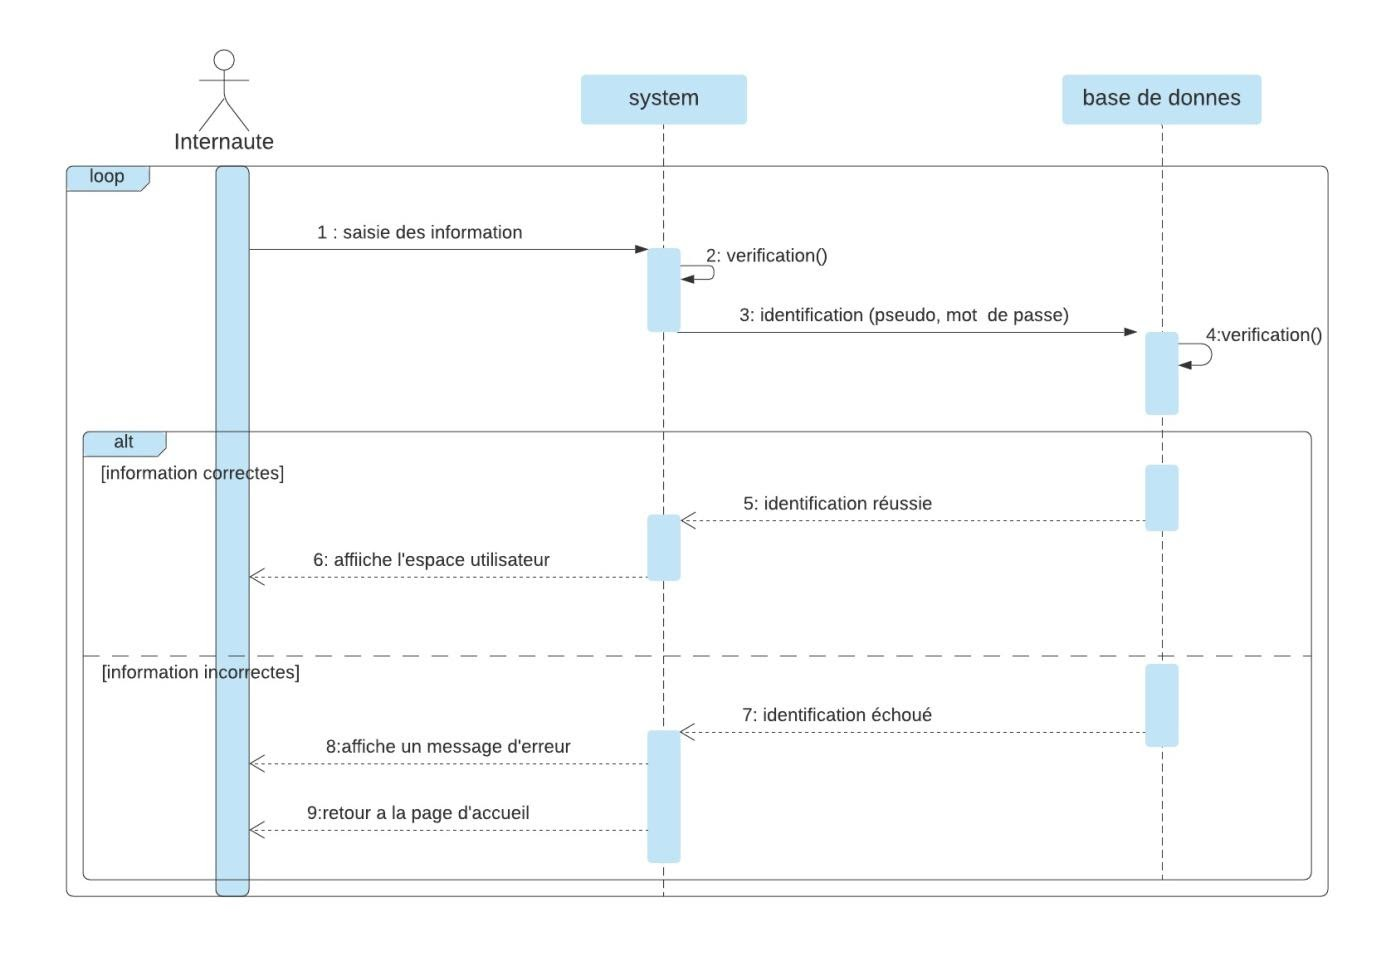
\includegraphics[width=1\textwidth]{images/sequence diag authentification.jpg}
            \caption{Diagramme de séquence du cas d'utilisation "Connexion".}
            \label{fig:my_label}
        \end{figure}
        
\begin{itemize}
\item  \textbf{Publication de service}
\end{itemize}
	Le diagramme de séquence suivant illustre les interactions nécessaires pour la publication d'un service.
	Après l'authentification, le fournisseur peut déposer un service tout en remplissant un formulaire de 
	dépôt d'un service. Si le fournisseur oublie de remplir l'un des champs ou remplit un champ dans une case 
	inapproprié le service ne sera pas publié.
	
    \begin{figure}[H]
            \centering
            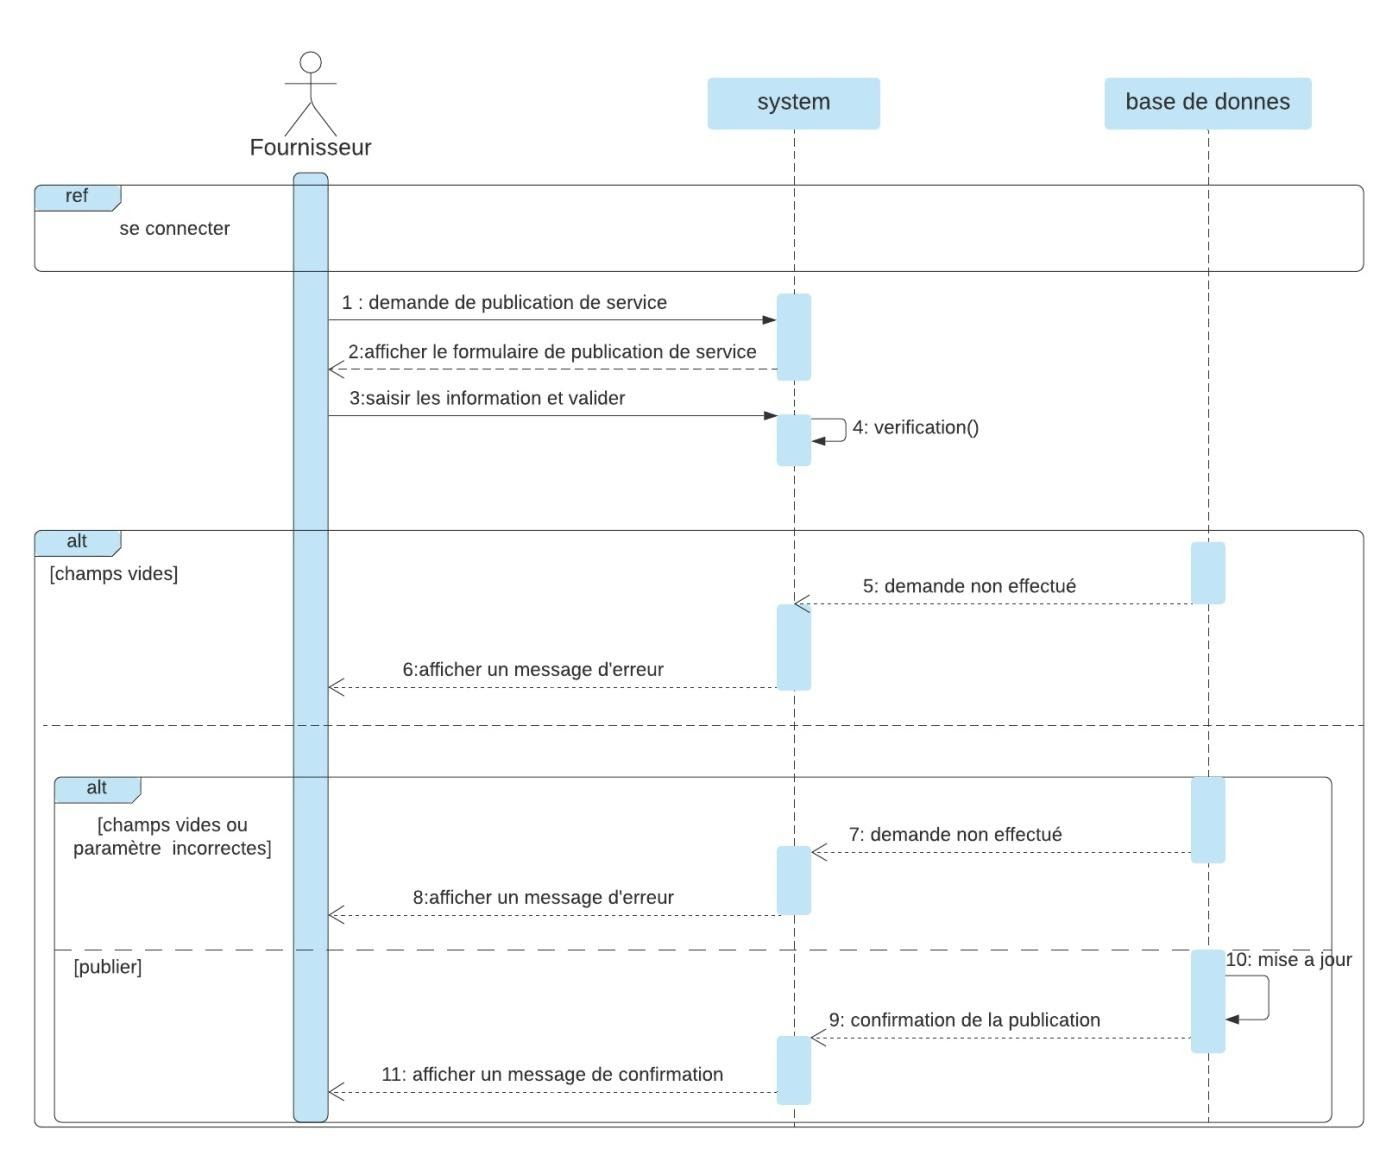
\includegraphics[width=1\textwidth]{images/sequence diag publier service.jpg}
            \caption{Diagramme de séquence du cas d'utilisation "Publication de service".}
            \label{fig:my_label}
    \end{figure}
        
\begin{itemize}
\item \textbf{Recherche de service}
\end{itemize}
    Le diagramme de séquence suivant illustre les interactions nécessaires pour la recherche d'un service. En effet,
    l'utilisateur saisit les critères de recherche, le système vérifie alors si le service recherché existe dans la
    base de données ou pas, et lui affiche un résultat.
        
    \begin{figure}[H]
            \centering
            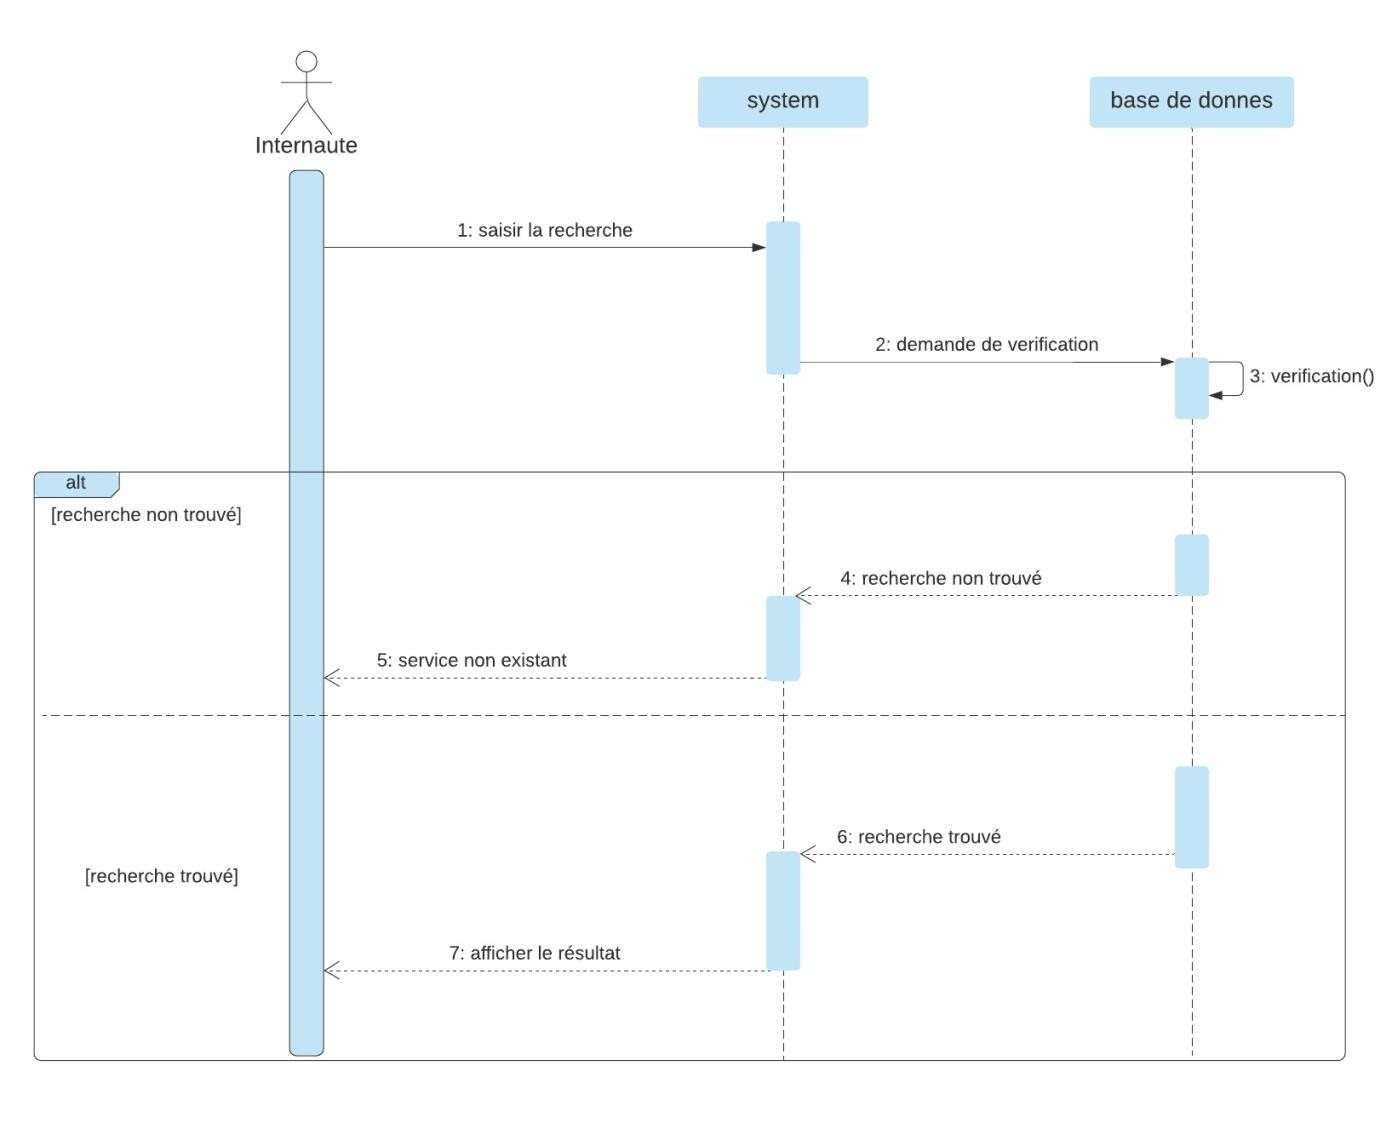
\includegraphics[width=1\textwidth]{images/sequence diag recherche service.jpg}
            \caption{Diagramme de séquence du cas d'utilisation "Recherche de service".}
            \label{fig:my_label}
    \end{figure}

\begin{itemize}
\item \textbf{Suppression de service}
\end{itemize}

    Le diagramme de séquence suivant illustre les interactions nécessaires pour la suppression d'un service. En effet,
    le fournisseur choisit un service, le système lui demande une confirmation de suppression, si oui, le système 
    vérifie l'existence de service dans la base de données, si le service existe alors la suppression va être appliquée,
    sinon un message d'erreur va être affiché.
        
    \begin{figure}[H]
            \centering
            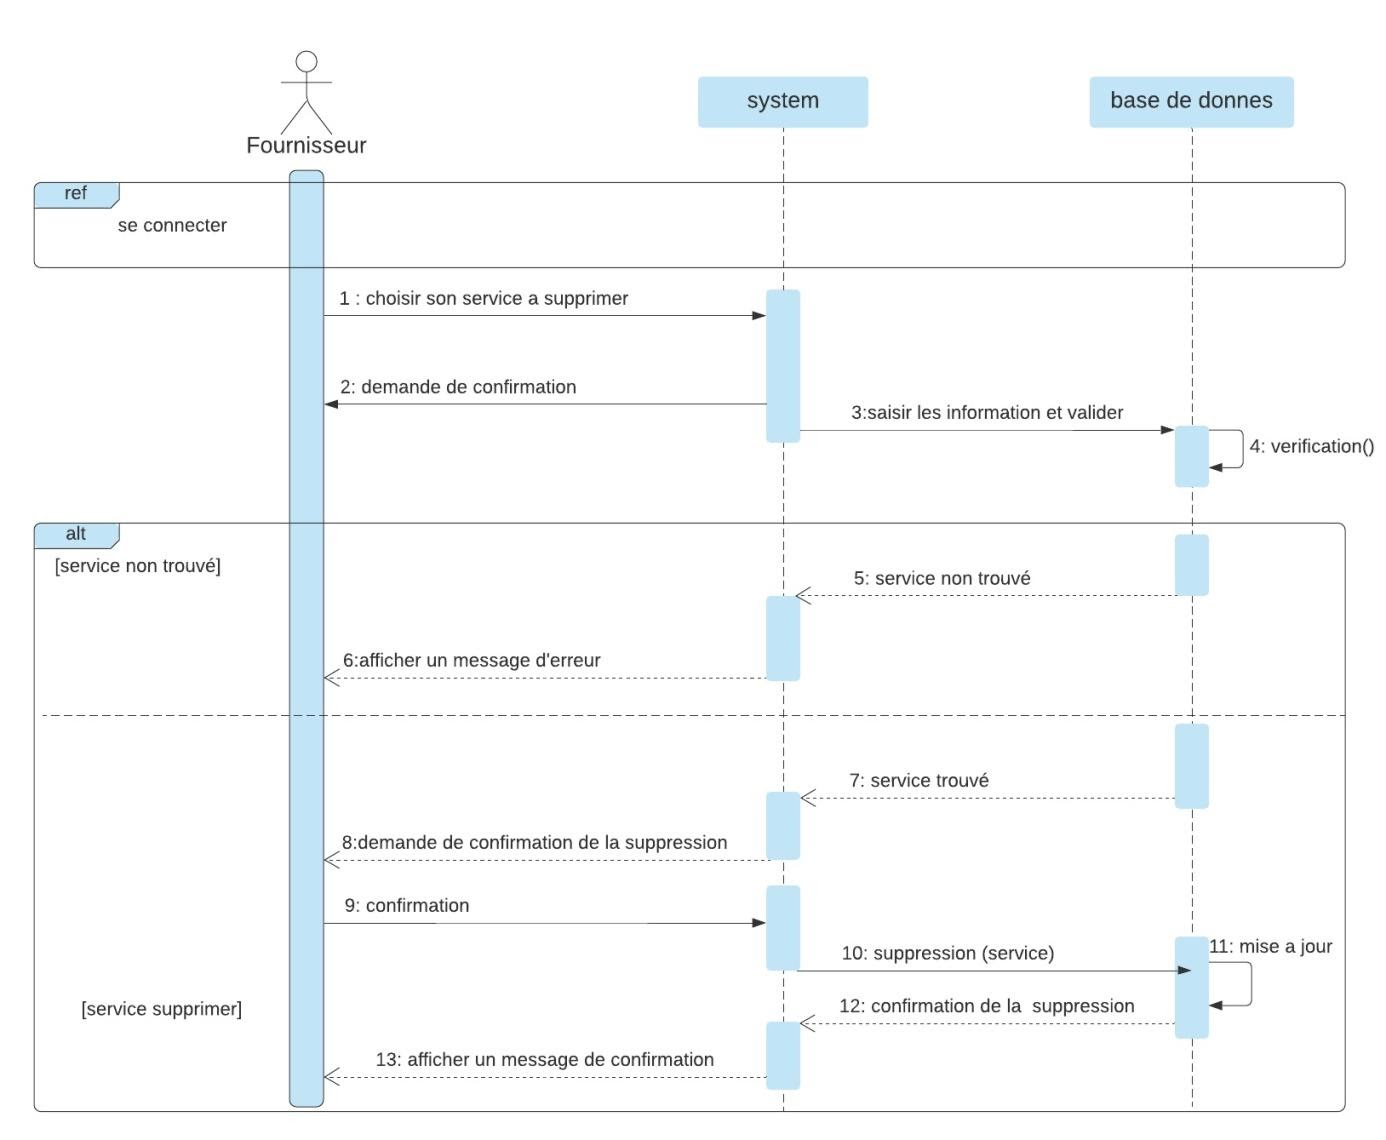
\includegraphics[width=1\textwidth]{images/sequence diag supp service.jpg}
            \caption{Diagramme de séquence du cas d'utilisation "Suppression de service".}
            \label{fig:my_label}
    \end{figure}
        
        \begin{itemize}
            \item \textbf{Modification de compte}
        \end{itemize}
        Le diagramme de séquence suivant illustre les interactions nécessaires pour qu'un fournisseur modifie les 
	informations de son compte. En effet, le fournisseur  demande au système la modification de son compte,
	ensuite le système affiche le formulaire de modification et le fournisseur  modifie ses informations,
	le système vérifie à nouveau les informations, si elles sont correctes, la base de données sera 
	mise à jour sinon un message d'erreur sera affiché.
    
        \begin{figure}[H]
            \centering
            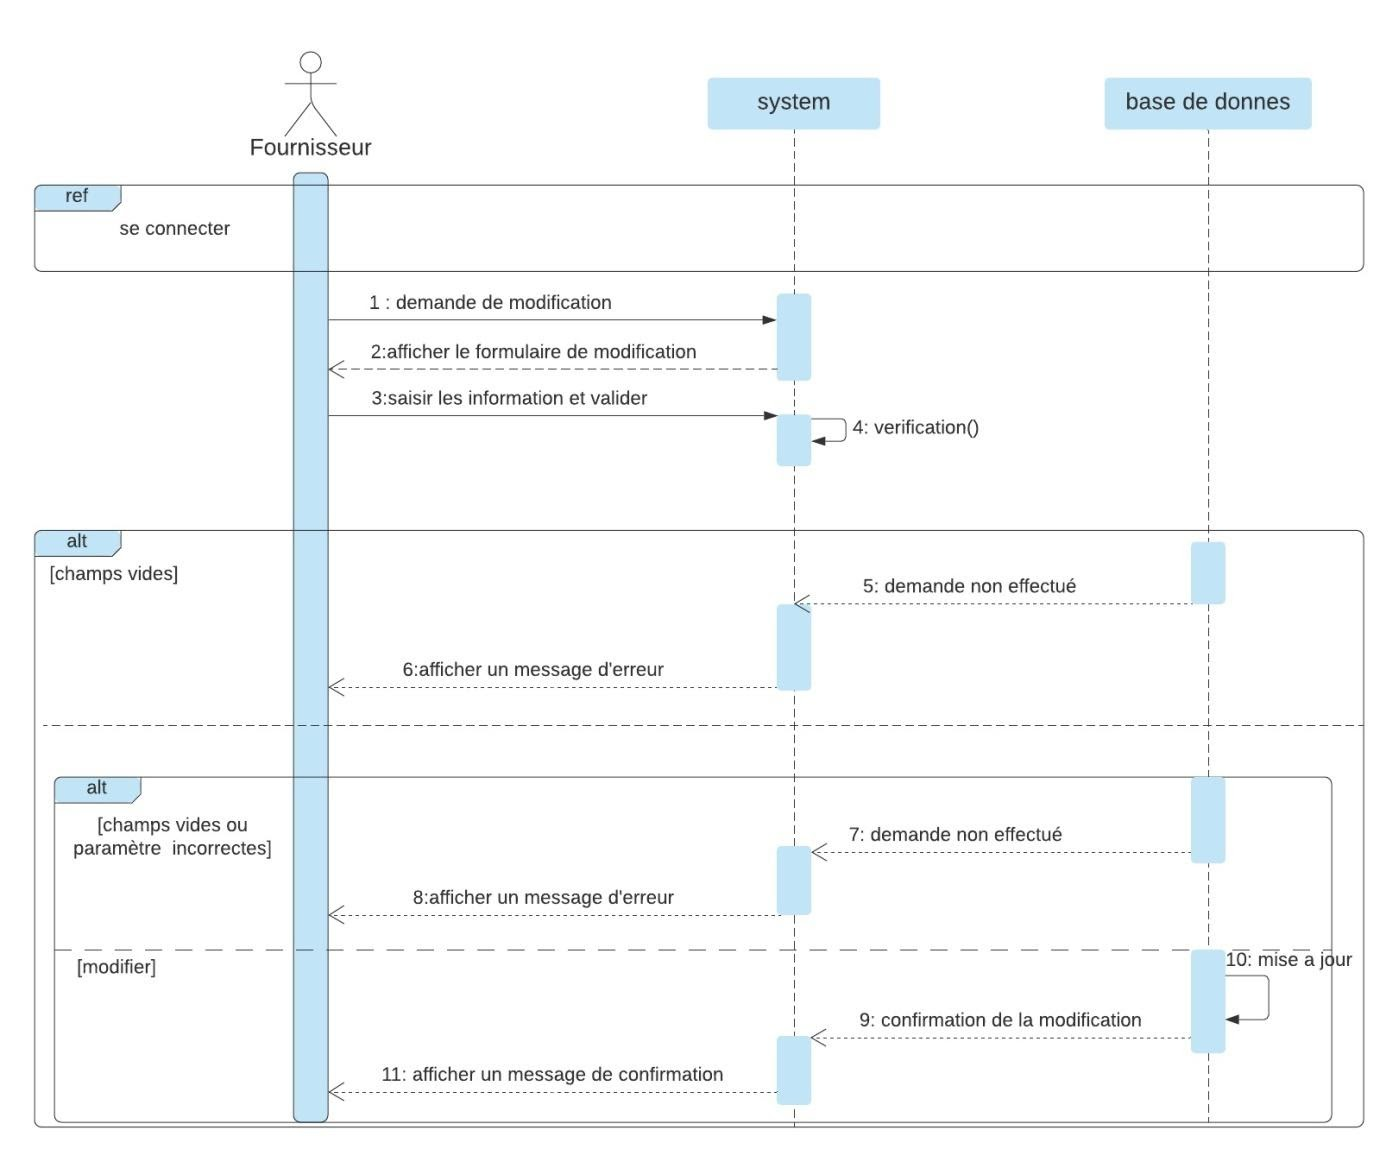
\includegraphics[width=1\textwidth]{images/sequence diag modifier compte.jpg}
            \caption{Diagramme de séquence du cas d'utilisation "Modification de compte".}
            \label{fig:my_label}
        \end{figure}
        
        \begin{itemize}
            \item \textbf{Suppression d'un utilisateur}
        \end{itemize}
        Le diagramme de séquence suivant illustre les interactions nécessaires pour la suppression d'un utilisateur.
	En effet, l'administrateur choisit l'utilisateur à supprimer, le système vérifie son existence dans la base de données,
	si l'utilisateur existe la suppression sera appliquée sinon un message d'erreur sera affiché.
        
        \begin{figure}[H]
            \centering
            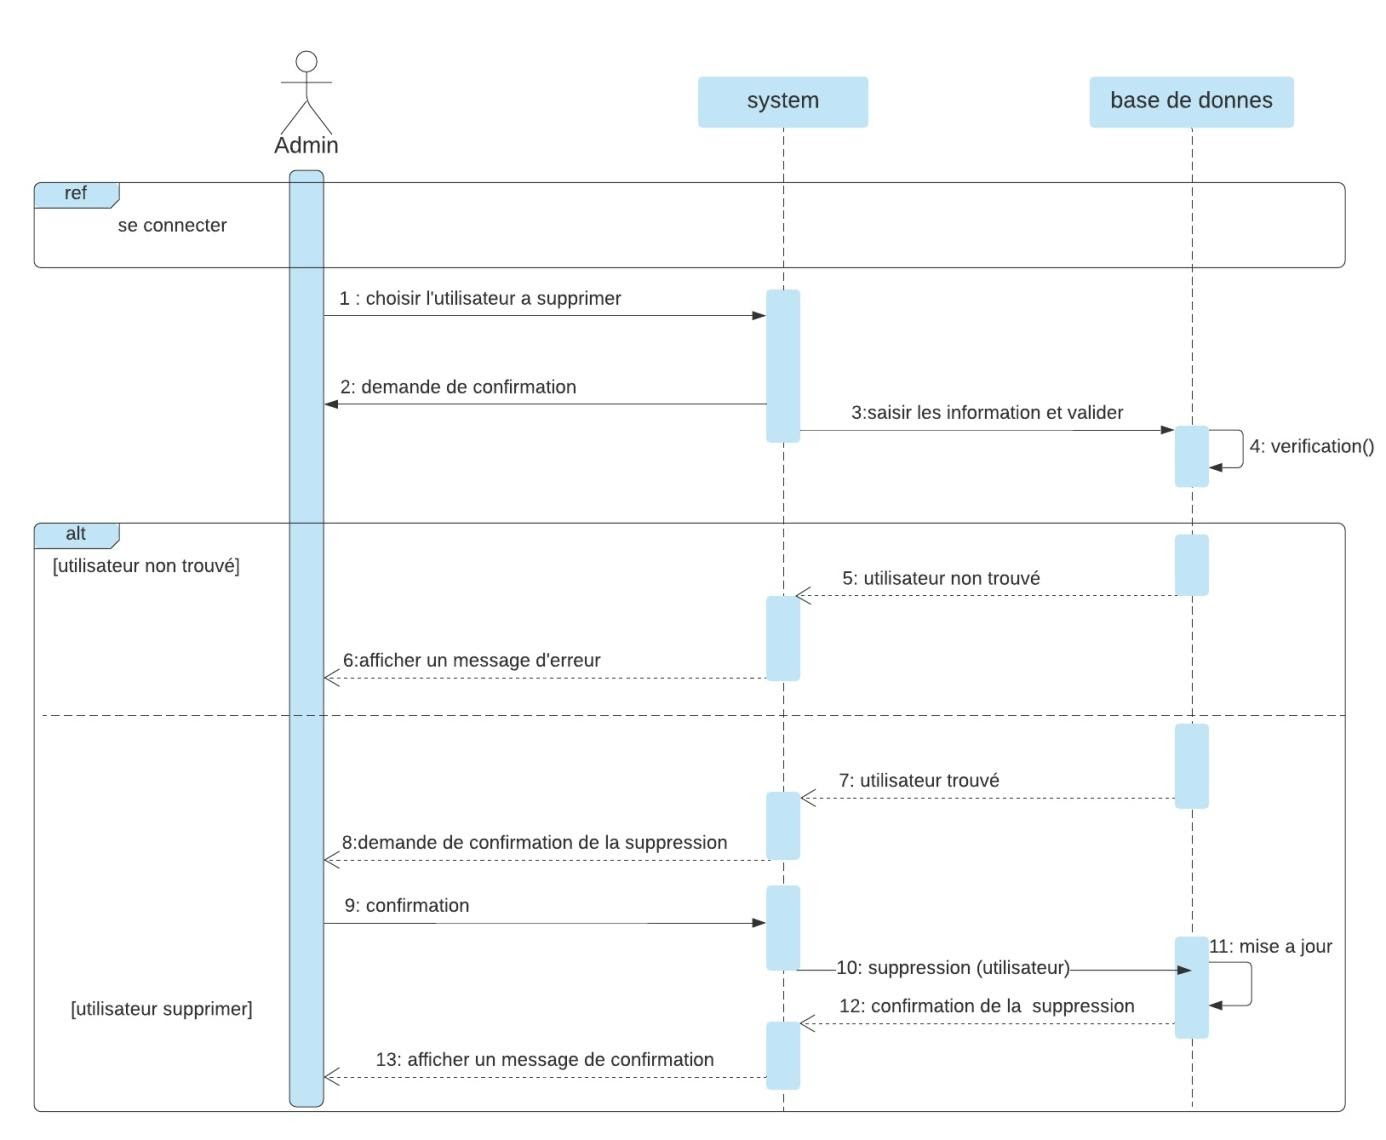
\includegraphics[width=1\textwidth]{images/sequence diag supp user.jpg}
            \caption{Diagramme de séquence du cas d'utilisation "Suppression d'un utilisateur".}
            \label{fig:my_label}
        \end{figure}
        
        \subsection{Diagramme de classes}
        Le digramme de classes permet de donner la représentation statique du système à développer. 
	Cette représentation est centrée sur les concepts de classe et d'association. 
	Chaque classe se décrit par les données et les traitements dont elle est responsable.
	Nous avons pu construire le diagramme de classes indiqué ci-dessous ensuite le passage au modèle 
	logique est effectué pour former la base de données de notre application.
          \begin{figure}[H]
            \centering
            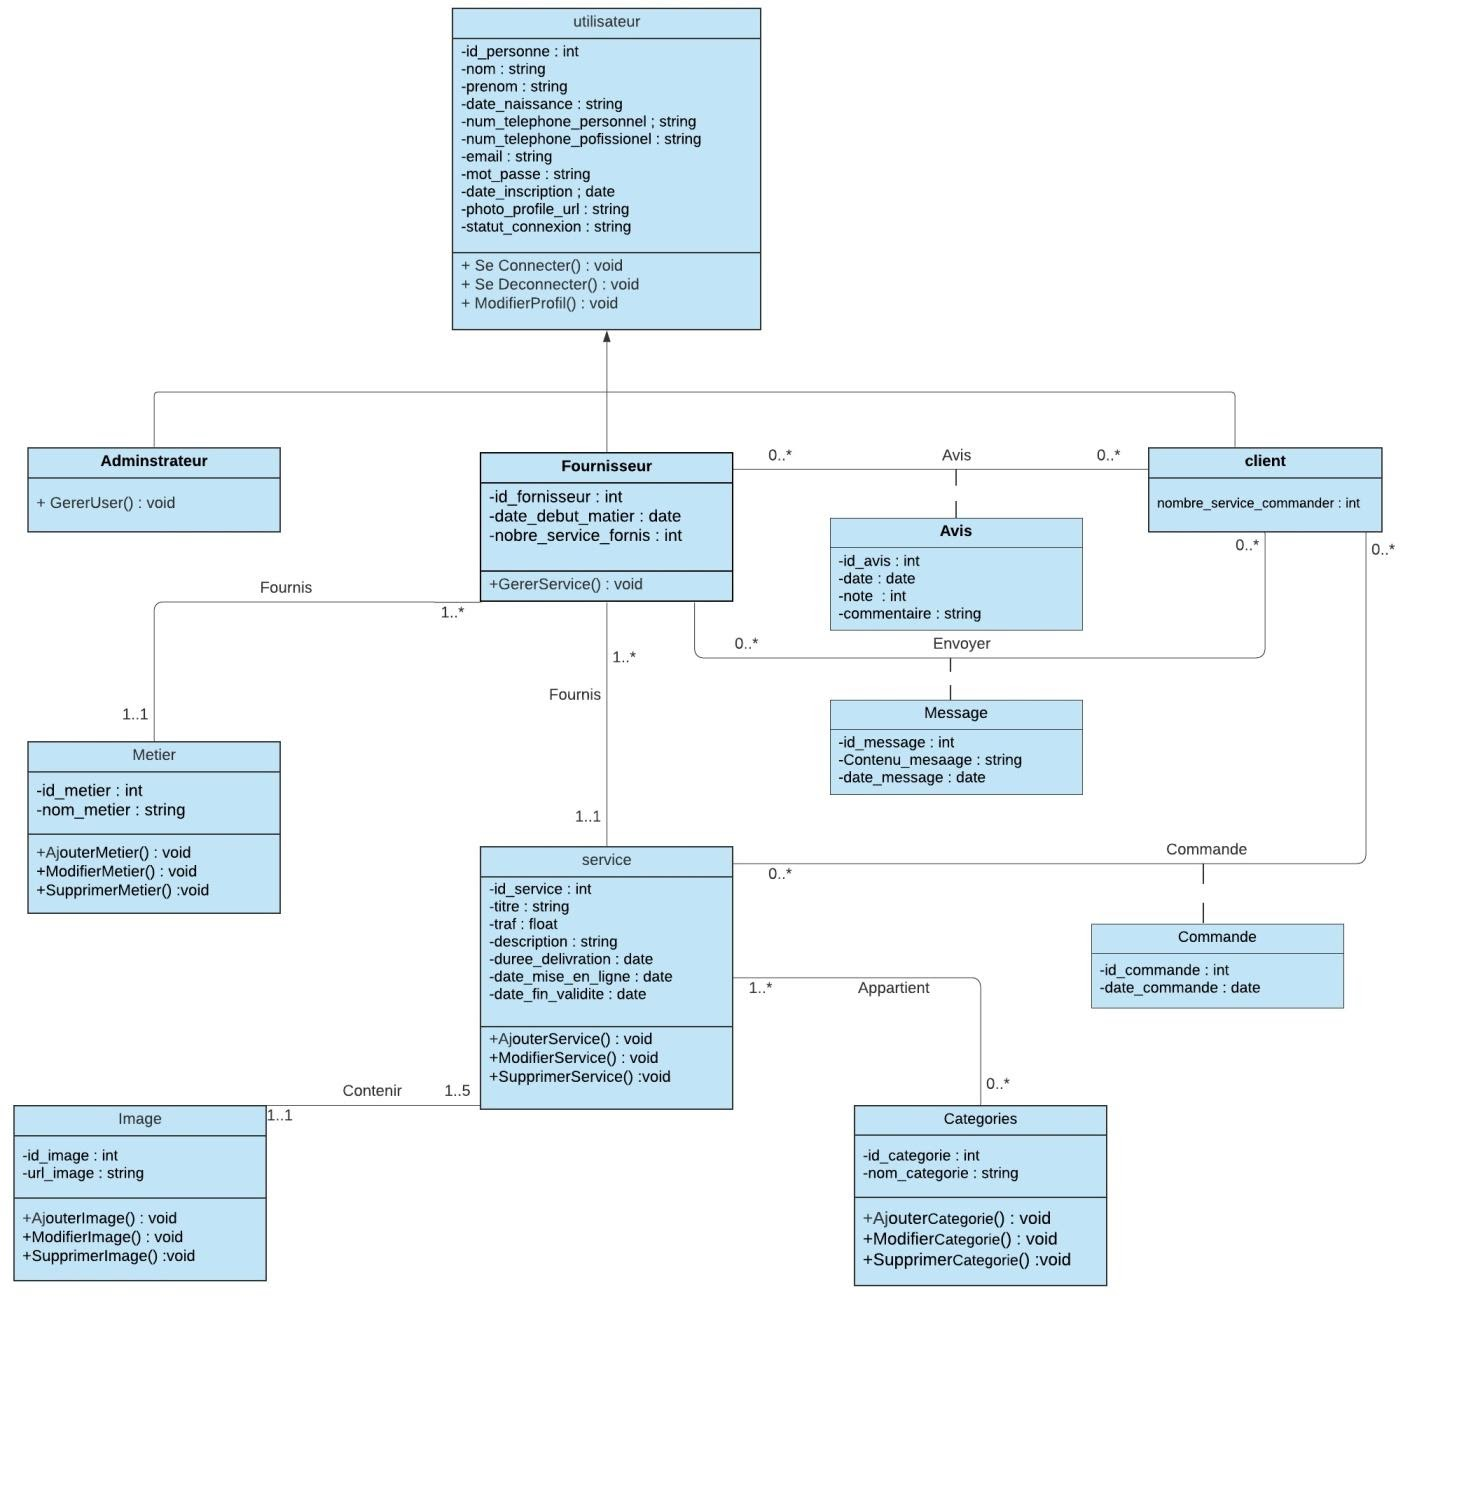
\includegraphics[width=1\textwidth]{images/Diag de classe.jpg}
            \caption{Diagramme de classes.}
            \label{fig:my_label}
        \end{figure}

        \subsection{Schéma relationnel}
        Pour réaliser ce passage, nous avons suivi des règles strictes et précises permettant 
	de traduire le contenu conceptuel du diagramme de classes en modèle relationnel.

            \subsubsection{Règle de passage du diagramme de classes au modèle relationnel}
            Nous avons pu passer du diagramme de classes au modèle relationnel en se basant sur les règles suivantes :
            \begin{itemize}
                \item \textbf{Règle 1}
                
                Transformation des classes : Chaque classe devient une table. L'identifiant de la classe
		devient la clé primaire et chaque attribut de classe se transforme en un champ de table.
                
                \item \textbf{Règle 2}
                
                Association plusieurs-à-plusieurs : Toute association sous forme (?..*) à (?..*), 
		donne naissance à trois tables, dont la table dérivée de l'entité association possédera
		les clés primaires des deux autres tables comme clé primaire, plus ses propres attributs 
		s'il s'agit d'une classe d'association.

                \item \textbf{Règle 3}
                
                Association un-à-plusieurs : Toute association binaire (?..1) à (?..*) donne naissance à
		une table dérivée de l'entité de la cardinalité (1..1), et sa clé primaire est déposé comme
		clé étrangère dans la table dérivée de l'entité de la cardinalité (?..*).
            \end{itemize}
            
            \subsubsection{Le modèle logique de données}
           \begin{figure}[H]
            \centering
            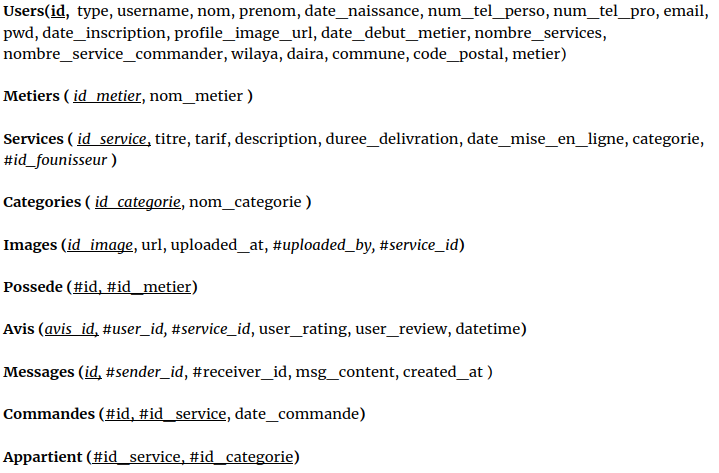
\includegraphics[width=1\textwidth]{images/MLD.png}
            \caption{Modèle logique de données.}
            \label{fig:my_label}
        \end{figure}
        
        \subsection{Conclusion}
        Dans ce chapitre, nous avons présenté le processus de développement UP, le langage de modélisation UML,
	et fait la modélisation des différents diagrammes : diagrammes de cas d'utilisation,
	diagrammes de séquence et diagramme de classes. Cette étape de modélisation nous a permis
	d'avoir une vue générale sur le comportement théorique des fonctionnalités offertes par
	notre application. Cette base théorique nous servira de guide pour le développement de
	l'application, qui fera l'objet du chapitre suivant.

%Fin du chapitre 2

%Début du chapitre 3

\chapter{Réalisation et implémentions}

\section{Introduction}

Depuis le début de ce projet, nous avons bien déterminé les perspectives de
l'application en commençant par une étude préalable, qui nous a permis d'avoir
un objectif bien concret. Puis en arrivant à l'analyse, nous avons pu avoir une
idée bien claire sur comment va être notre application web, et c'est ce qui nous
a mené à mieux comprendre ses fonctionnalités. Dans ce chapitre, nous allons
nous appuyer sur la conception réalisée dans le chapitre précédent afin de
présenter la concrétisation de l'application à travers son implémentions. Nous
allons commencer par présenter les différents langages de développement ainsi
que les outils de travail utilisés dans notre démarche, nous allons ensuite
présenter en détail le principe de fonctionnement de ses outils, nous allons
finir en présentant les interfaces des pages web de notre application ainsi que
les différentes actions possibles à effectuer dans ces pages.
    
\section{Outils et environnement de développement}

\subsection{XAMPP}

XAMPP est l'environnement de développement PHP le plus populaire (\rmq{sous
windows}). XAMPP est une distribution Apache entièrement gratuite et facile à
installer contenant MySQL, PHP et Perl. Le paquetage open source XAMPP a été mis
au point pour être incroyablement facile à installer et à utiliser.

\begin{figure}[H]
    \centering
    
\includegraphics[width=0.5\textwidth]{images/1024px-Xampp_logo.svg.png}
    \caption{Logo de XAMPP}
    \label{fig:my_label}
\end{figure}
        
\subsection{MYSQL}
        
MySQL est un système de gestion de base de données relationnel, un langage de
requêtes vers les bases de données exploitant le modèle relationnel et utilise
le langage SQL comme langage de requête. SQL est un langage de manipulation de
bases de données mis au point dans la années 70 par IBM, il permet d'exécuter
trois types de manipulations :

\begin{enumerate}
    \item La manipulation des tables : Création, suppression, modification de la
        structure.
    \item Les manipulations des données de la base : Sélection, modification,
        suppression d'enregistrement.
    \item La gestion des droits d'accès aux tables : Contrôle des données, droit
        d'accès, validation des modifications. \cite{memoire}
\end{enumerate}

\begin{figure}[H]
    \centering
    
\includegraphics[width=0.5\textwidth]{images/1200px-MySQL.svg.png}
    \caption{Logo de MySQL}
    \label{fig:my_label}
\end{figure}

\subsection{IDE Visual Studio Code}

Visual Studio Code est un éditeur de code extensible développé par Microsoft
pour Windows, Linux et macOS. Les fonctionnalités incluent la prise en charge du
débogage, la mise en évidence de la syntaxe, la complétion intelligente du code,
les snippets, la refactorisation du code et Git intégré. \cite{ide}

\begin{figure}[H]
    \centering
    
\includegraphics[width=0.3\textwidth]{images/1024px-Visual_Studio_Code_1.35_icon.svg.png}
    \caption{Logo de VS Code}
    \label{fig:my_label}
\end{figure}

\subsection{Draw.io}

C'est une application gratuite en ligne, accessible via le navigateur qui permet
de dessiner des diagrammes ou des organigrammes. Cet outil nous propose de
concevoir toutes sortes de diagrammes, de dessins vectoriels, de les enregistrer
ou de les exporter en format image, XML,PDF, etc.

\begin{figure}[H]
    \centering
    
\includegraphics[width=0.5\textwidth]{images/drawio.jpg}
    \caption{Logo de Draw.io}
    \label{fig:my_label}
\end{figure}

\subsection{Git}

Git est un logiciel de gestion de versions décentralisé. C'est un logiciel libre
créé par Linus Torvalds, auteur du noyau Linux, et distribué selon les termes de
la licence publique générale GNU version 2. Le principal contributeur actuel de
git et depuis plus de 16 ans est Junio C Hamano. En 2016, il s'agit du logiciel
de gestion de versions le plus populaire qui est utilisé par plus de douze
millions de personnes.

\begin{figure}[H]
    \centering
    
\includegraphics[width=0.5\textwidth]{images/1280px-Git-logo.svg.png}
    \caption{Logo de Git}
    \label{fig:my_label}
\end{figure}

\subsection{Langages de programmation}

\subsubsection{HTML}

HTML signifie « HyperText Markup Language » qu'on peut traduire par « langage de
balises pour l'hypertexte ». Il est utilisé afin de créer et de représenter le
contenu d'une page web et sa structure. D'autres technologies sont utilisées
avec HTML pour décrire la présentation d'une page (CSS) et/ou ses
fonctionnalités interactives (JavaScript).\cite{html}

HTML fonctionne grâce à des « balises » qui sont insérées au sein d'un texte
normal. Chacune de ces balises indique la signification de telle ou telle
portion de texte dans le site, par exemple <head>, <title>, <body>, <header>,
<footer>, <article>, <section>, <p>, <div>, <span>, <img> et bien d'autres
encore. Ces éléments forment les blocs utilisés pour construire un site
web.\cite{html}

On parle d'« hypertexte » en référence aux liens qui connectent les pages web
entre elles. \cite{html}

\subsubsection{CSS }

Cascading Style Sheets (CSS) est un langage de feuille de style utilisé pour
décrire la présentation d'un document écrit en HTML ou en XML. CSS décrit la
façon dont les éléments doivent être affichés à l'écran, sur du papier, en
vocalisation, ou sur d'autres supports.\cite{css}

CSS est l'un des langages principaux du Web ouvert et a été standardisé par le
W3C. Ce standard évolue sous forme de niveaux (levels), CSS1 est désormais
considéré comme obsolète, CSS2.1 correspond à la recommandation et CSS3, qui est
découpé en modules plus petits, est en voie de standardisation.\cite{css}

\subsubsection{JavaScript}

JavaScript (qui est souvent abrégé en « JS ») est un langage de script léger,
orienté objet, principalement connu comme le langage de script des pages web.
Mais il est aussi utilisé dans de nombreux environnements extérieurs aux
navigateurs web tels que Node.js, Apache CouchDB voire Adobe Acrobat. \cite{js}

Il est développé par Netscape et utilisé dans des millions de pages web et
d'applications serveur dans le monde entier.\cite{js}

Contrairement à une conception populaire, JavaScript n'est pas « du Java
interprété ». En quelques mots, JavaScript est un langage de script dynamique
utilisant une construction d'objets basée sur des prototypes.\cite{js}

\subsubsection{PHP }

PHP (Hypertext Preprocessor) est un langage de script Web intégré au HTML. Cela
signifie que le code PHP peut être inséré dans le code HTML d'une page Web.
\cite{php}

Lors de l' accès à une page PHP , le code PHP est lu ou "analysé" par le serveur
sur lequel la page réside. Les résultats des fonctions PHP de la page sont
généralement renvoyés sous forme de code HTML, qui peut être lu par le
navigateur.\cite{php}

Étant donné que le code PHP est transformé en HTML avant le chargement de la
page, les utilisateurs ne peuvent pas afficher le code PHP sur une page. Cela
rend les pages PHP suffisamment sécurisées pour accéder aux bases de données et
autres informations sécurisées.\cite{php}

\subsubsection{Framworks et Bibliothèques utilisé}

Un Framework est, comme son nom l'indique en anglais, un «  cadre de travail » .
L'objectif d'un Framework est généralement de simplifier le travail des
développeurs informatiques, en leur offrant une architecture "prête à l'emploi"
et qui leur permettre de ne pas repartir de zéro à chaque nouveau projet.

Les Frameworks sont comparables aux patrons de couture. Les principaux avantages
sont donc :

\begin{itemize}
    \item La réutilisation des codes.
    \item La standardisation de la programmation.
    \item La formalisation d'une architecture adaptée aux besoins de chaque
        entreprise.
\end{itemize}

À noter aussi que les Frameworks sont toujours « enrichis » de l'expérience de
tous les développements antérieurs.

Nous avons utilisé deux Frameworks :

\subsubsection{Codeigniter 4}

CodeIgniter est un framework de développement d'applications - une boîte à
outils - pour les personnes qui créent des sites Web en utilisant PHP. Son
objectif est de vous permettre de développer des projets beaucoup plus
rapidement que si vous écriviez du code à partir de zéro, en fournissant un
riche ensemble de bibliothèques pour les tâches courantes, ainsi qu'une
interface simple et une structure logique pour accéder à ces bibliothèques.
CodeIgniter vous permet de vous concentrer de manière créative sur votre projet
en minimisant la quantité de code nécessaire pour une tâche donnée.

Dans la mesure du possible, CodeIgniter est resté aussi flexible que possible,
vous permettant de travailler comme vous le souhaitez, sans être obligé de
travailler d'une certaine manière. Le cadre peut avoir des pièces de base
facilement étendues ou complètement remplacées pour que le système fonctionne
comme vous en avez besoin. En bref, CodeIgniter est le framework malléable qui
essaie de fournir les outils dont vous avez besoin tout en restant à l'écart.

\begin{figure}[H]
    \centering
    
\includegraphics[width=1\textwidth]{images/ci-new-logo-04-02.jpg}
    \caption{Logo de CodeIgniter}
    \label{fig:my_label}
\end{figure}

CodeIgniter  requière l'installation d'un gestionnaire de dépendances « composer
».

Pour installer CodeIgniter  nous devons écrire dans le composer la commande
suivante :

\begin{figure}[H]
    \centering
    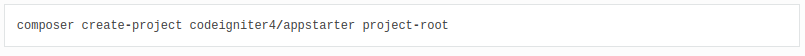
\includegraphics[width=1\textwidth]{images/codeigniter.png}
    \label{fig:my_label}
\end{figure}

\begin{itemize}
    \item \textbf{Organisation de Codeigniter}
    CodeIgniter  est composé d'une hiérarchie de dossiers et fichiers
        représentée dans cette figure :
    
    \begin{figure}[H]
        \centering
        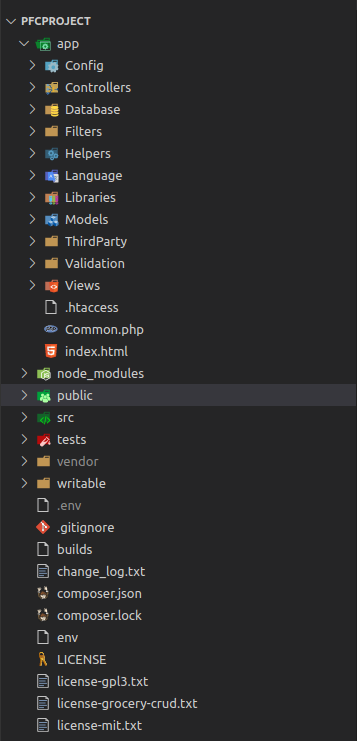
\includegraphics[width=0.7\textwidth]{images/ci structure.png}
        \caption{Structure de Codeigniter}
        \label{fig:my_label}
    \end{figure}

    \item \textbf{Les Controllers}
    
        La grande majorité des actions qu'un utilisateur enclenche mènera à
        l'appel d'une méthode d'un contrôleur. Les  Controllers   vont permettre
        de gérer les différentes actions demandées par les utilisateurs lors
        d'une action
    
    \begin{figure}[H]
        \centering
        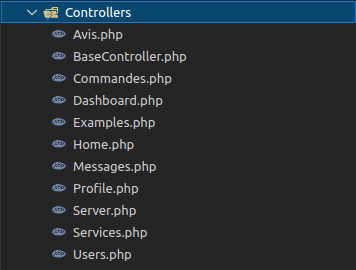
\includegraphics[width=0.7\textwidth]{images/controlers.png}
        \caption{Les controllers}
        \label{fig:my_label}
    \end{figure}
    
    \item \textbf{Les Models}
    \begin{itemize}
        \item  Le Model est la partie qui permet de stocker et de traiter les
            donnes.  D'une manière générale en PHP et avec CodeIgniter, le model
            n'effectue que les opérations en base de données.
        \item Pour créer un Modele avec CodeIgniter, il faut créer un fichier
            PHP dans le dossier system/application/models contenant une classe
            qui hérite de la classe Model du framework de CodeIgniter. Dans
            cette classe, on crée les fonctions qui effectuent les traitements
            sur les donnes et qui appellent les fonctions se chargeant de
            stocker les donnes (insertion SQL, écriture dans un fichier texte ou
            XML) ainsi qu'un constructeur appelant le constructeur de la classe
            Model.
    \end{itemize}

      \begin{figure}[H]
        \centering
        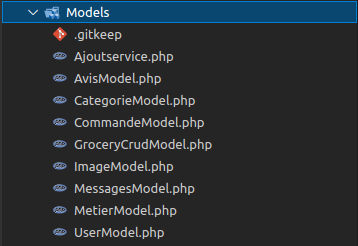
\includegraphics[width=0.7\textwidth]{images/models.png}
        \caption{Les Models}
        \label{fig:my_label}
    \end{figure}
    
    \item \textbf{Les Vues}
    
    Pour afficher correctement une page Web dans le navigateur, il faut utiliser
        une vue. C'est la vue qui est en charge de générer le code HTML.  Pour
        créer une vue avec CodeIgniter, il suffit de créer un script PHP ou
        HTML, qui affiche les donnes souhaites, dans le dossier
        system/application/views. Il n'y a pas de conventions particulières.
 
    \begin{figure}[H]
        \centering
        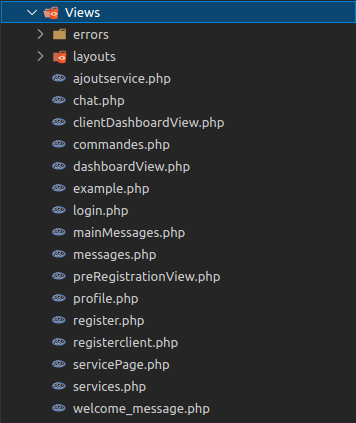
\includegraphics[width=0.7\textwidth]{images/viewq.png}
        \caption{Les Vues}
        \label{fig:my_label}
    \end{figure}
\end{itemize}
    

\subsubsection{TailwindCss}

Tailwind CSS se décrit lui-même comme un premier framework CSS utilitaire.
Plutôt que de se concentrer sur la fonctionnalité de l'élément stylisé, Tailwind
est centré sur la façon dont il doit être affiché. Cela permet au développeur de
tester plus facilement de nouveaux styles et de modifier la mise en page. Nous
interrogeons Jen Looper sur Tailwind et sur la façon dont cette approche peut
nous aider !

\begin{figure}[H]
    \centering
    
\includegraphics[width=1\textwidth]{images/tailwind-css-logo-vector.png}
    \caption{Logo de Tailwindcss}
    \label{fig:my_label}
\end{figure}

\subsubsection{La bibliothéque Grocery CRUD}

Grocery CRUD est une bibliothéque Open Source qui permet à l'aide du framework
Codeigniter de crée un panel administrateur facilement avec quelques lignes de
code.

\begin{figure}[H]
    \centering
    
\includegraphics[width=1\textwidth]{images/logo-big.png}
    \caption{Logo de GroceryCRUD}
    \label{fig:my_label}
\end{figure}

\begin{itemize}
    \item \textbf{Example :}
    Un exemple très simple pour commencer est les 4 lignes de code ci-dessous.
    Voici les fonctions les plus courantes :
    \begin{figure}[H]
    \centering
    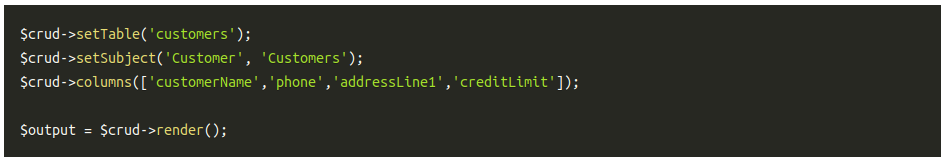
\includegraphics[width=1\textwidth]{images/example.png}
    \caption{Exemple d'utilisation de GroceryCrud}
    \label{fig:my_label}
\end{figure}
\end{itemize}

\section{Captures d'écran et fonctionnement}

\subsection{La page d'accueil}
    
La première interface que l'utilisateur rencontre lors de l'accès vers notre
application est celle de l'accueil. L'utilisateur aura deux choix, soit de se
connecter en cliquant sur le bouton "Connexion" s'il à déjà un compte, soit de
s'inscrire en cliquant sur le bouton "Inscription" si l'utilisateur n'a pas de
compte.

Si l'utilisateur choisi de se connecter, il sera rediriger vers l'interface
d'authentification, ou l'utilisateur sera amener a saisir ses information, dans
le cas ou ses informations sont correct, la page principale sera afficher, dans
le cas contraire, un message d'erreur sera afficher.

L'utilisateur en fonction de sont type (Admin, Fournisseur, Client) sera
automatiquement rediriger vers la page principale qui lui convient

\begin{figure}[H]
    \centering
    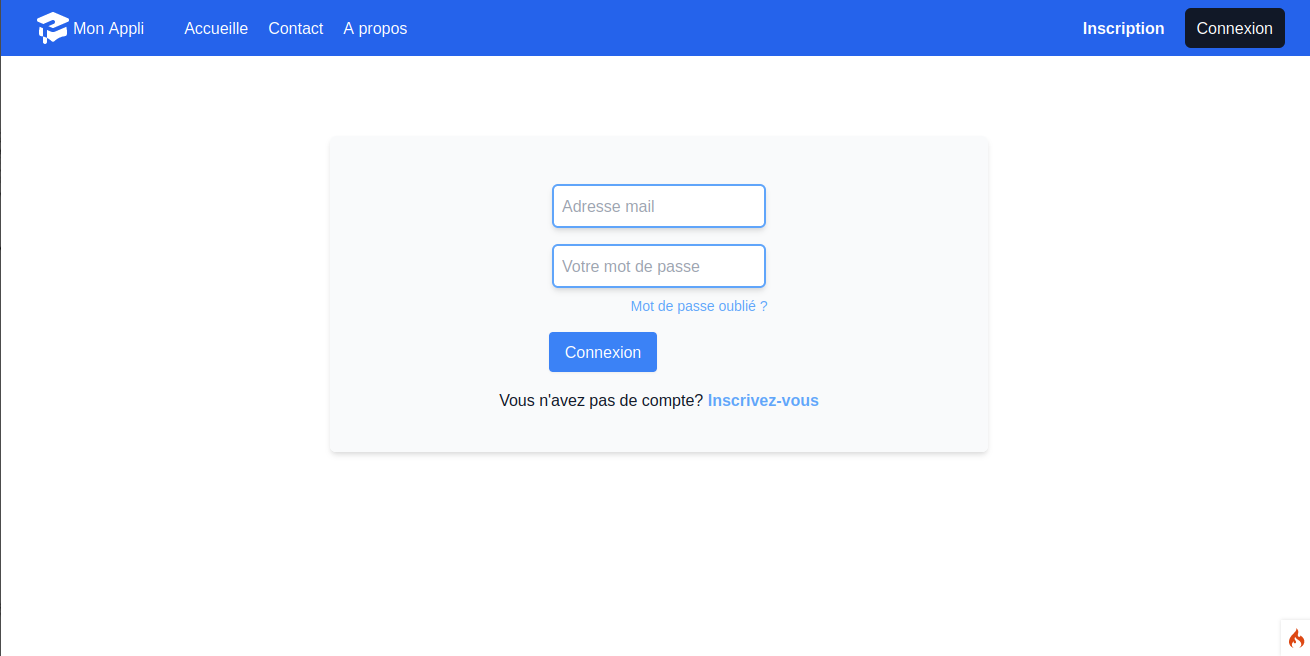
\includegraphics[width=1\textwidth]{images/accueil.png}
    \caption{Page d'accueil}
\end{figure}

\subsection{La page d'inscription}

Si l'utilisateur choisi de se s'inscrire, il sera rediriger vers l'interface
d'inscription, ou l'utilisateur sera amener remplir un formulaire d'inscription
en mentionnant son type au préalable, le système vas vérifier la validité des
informations saisie et les insèrent dans la base de donnée.

\begin{figure}[H]
    \centering
    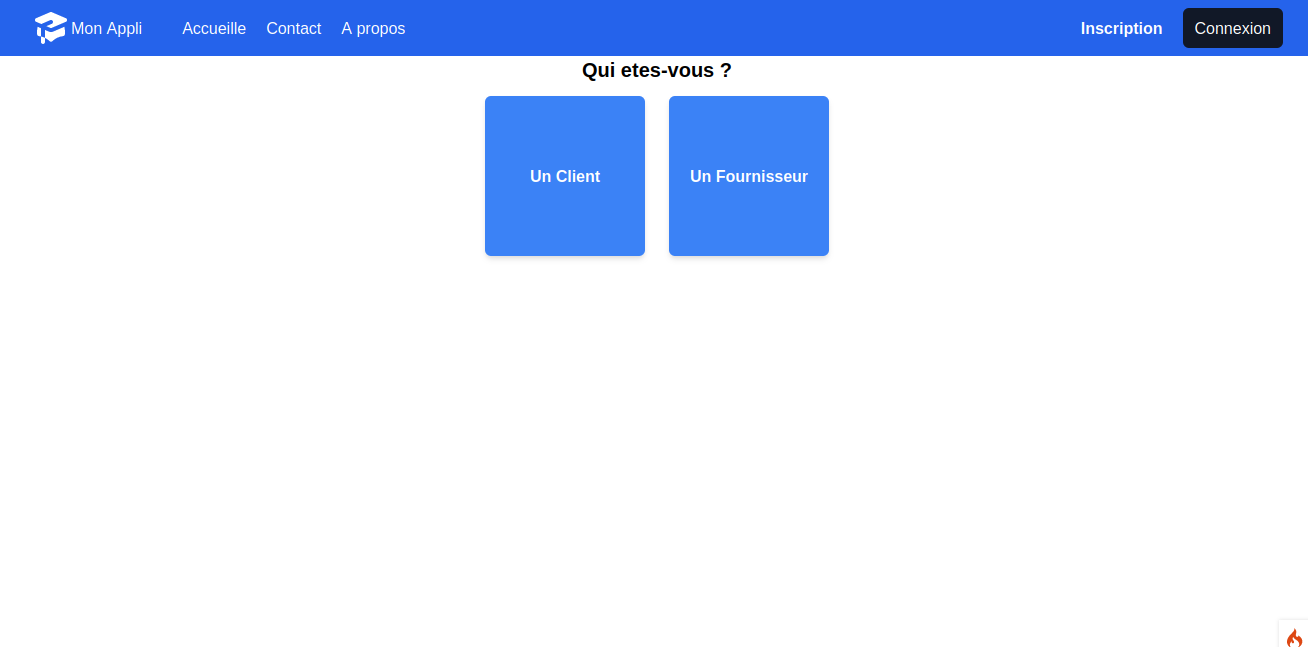
\includegraphics[width=1\textwidth]{images/inscription.png}
    \caption{Page de pré-inscription}
\end{figure}

\begin{figure}[H]
    \centering
    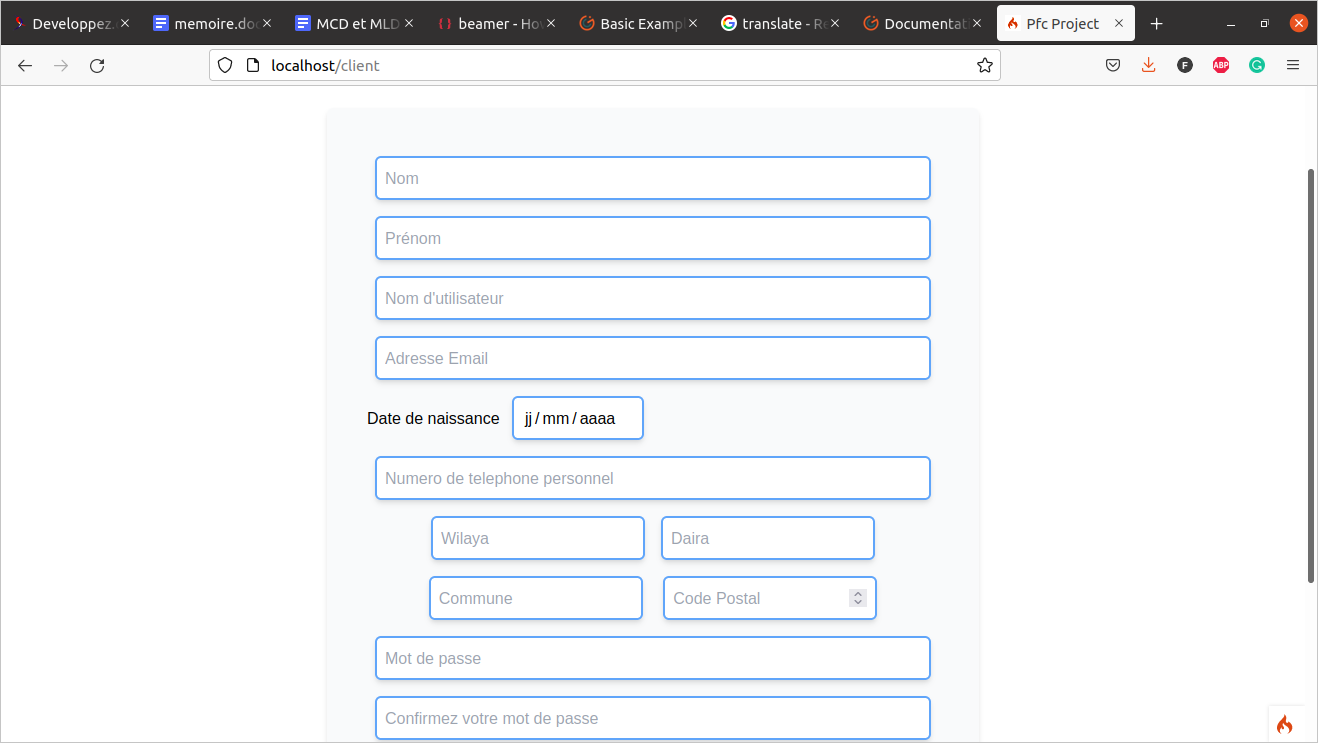
\includegraphics[width=1\textwidth]{images/formulaire.png}
    \caption{Formulaire d'inscription}
\end{figure}

\subsection{Interfaces coté client}

L'interface principale du client se présente comme suit :
\begin{figure}[H]
    \centering
    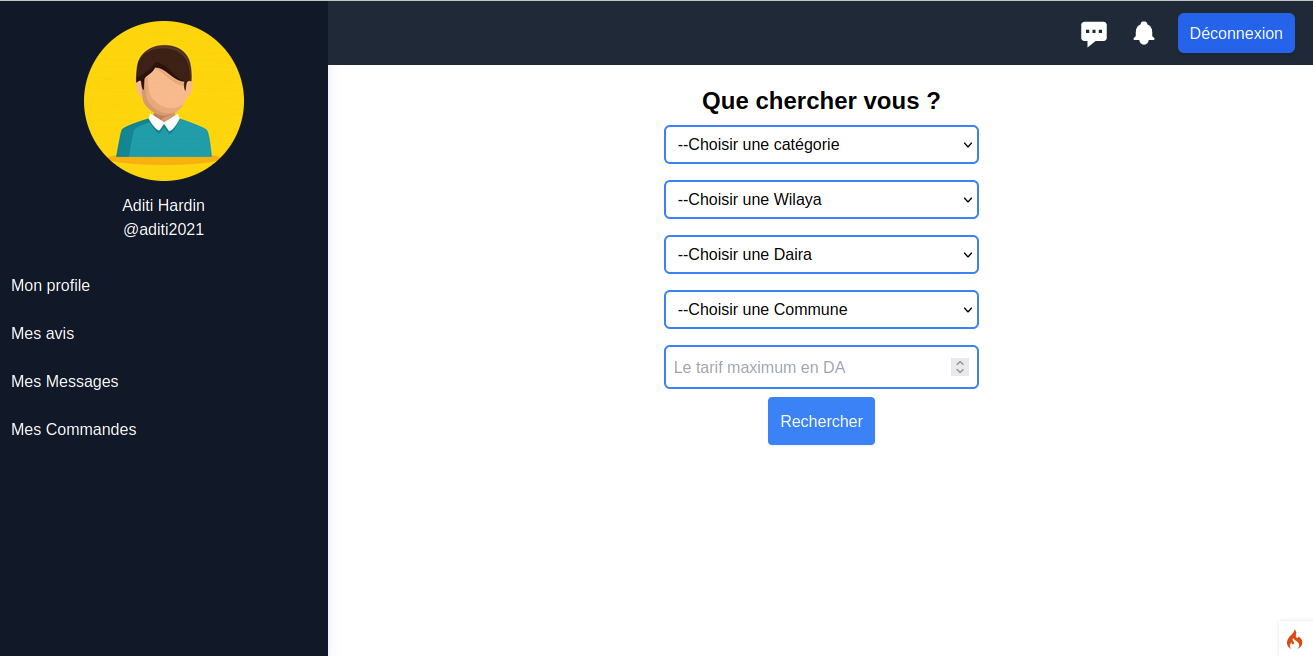
\includegraphics[width=1\textwidth]{images/client dash.png}
    \caption{Interface principale du client}
\end{figure}

Depuis cette interface, le client pourras :
\begin{itemize}
    \item Chercher des services selon un filtre
    \item Voir les messages échanger
    \item Voir les commandes effectuer et leurs état
    \item voir les avis précédemment laisser.
\end{itemize}

\begin{figure}[H]
    \centering
    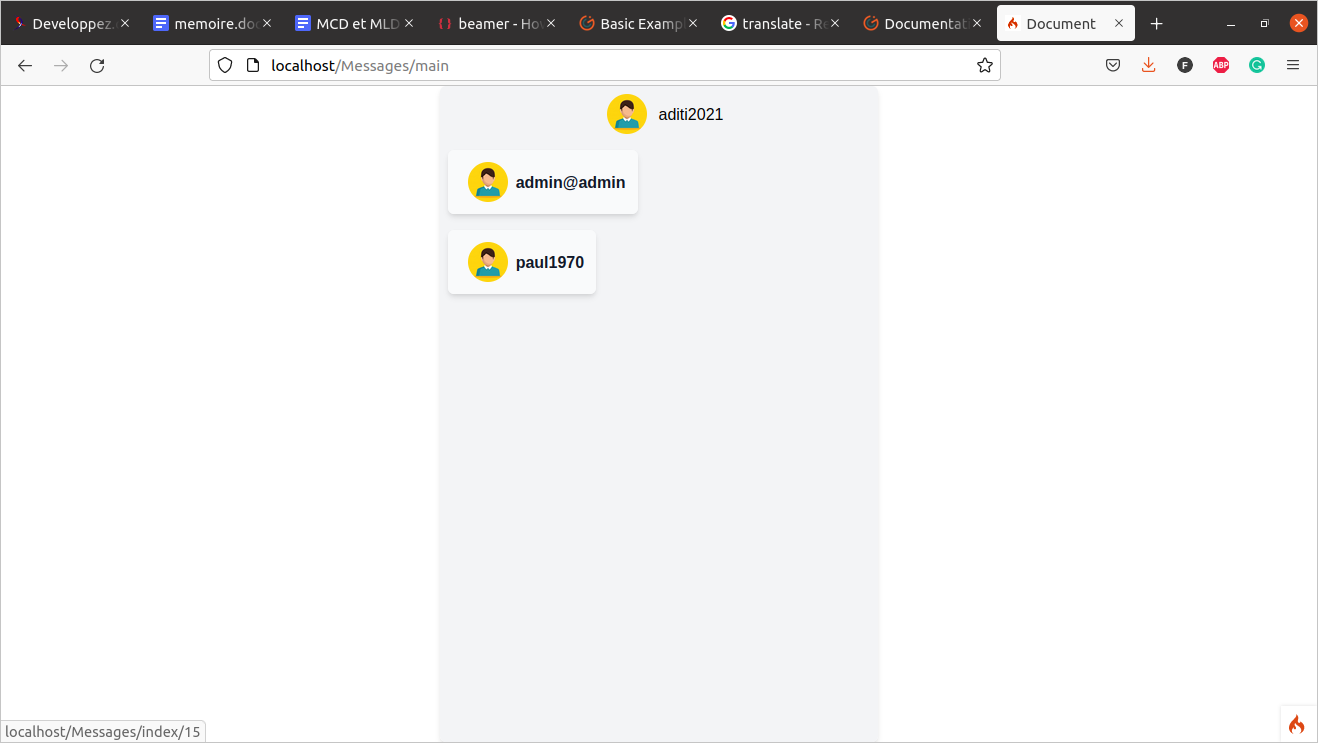
\includegraphics[width=1\textwidth]{images/messages.png}
    \caption{Interface des messages échanger}
\end{figure}

\begin{figure}[H]
    \centering
    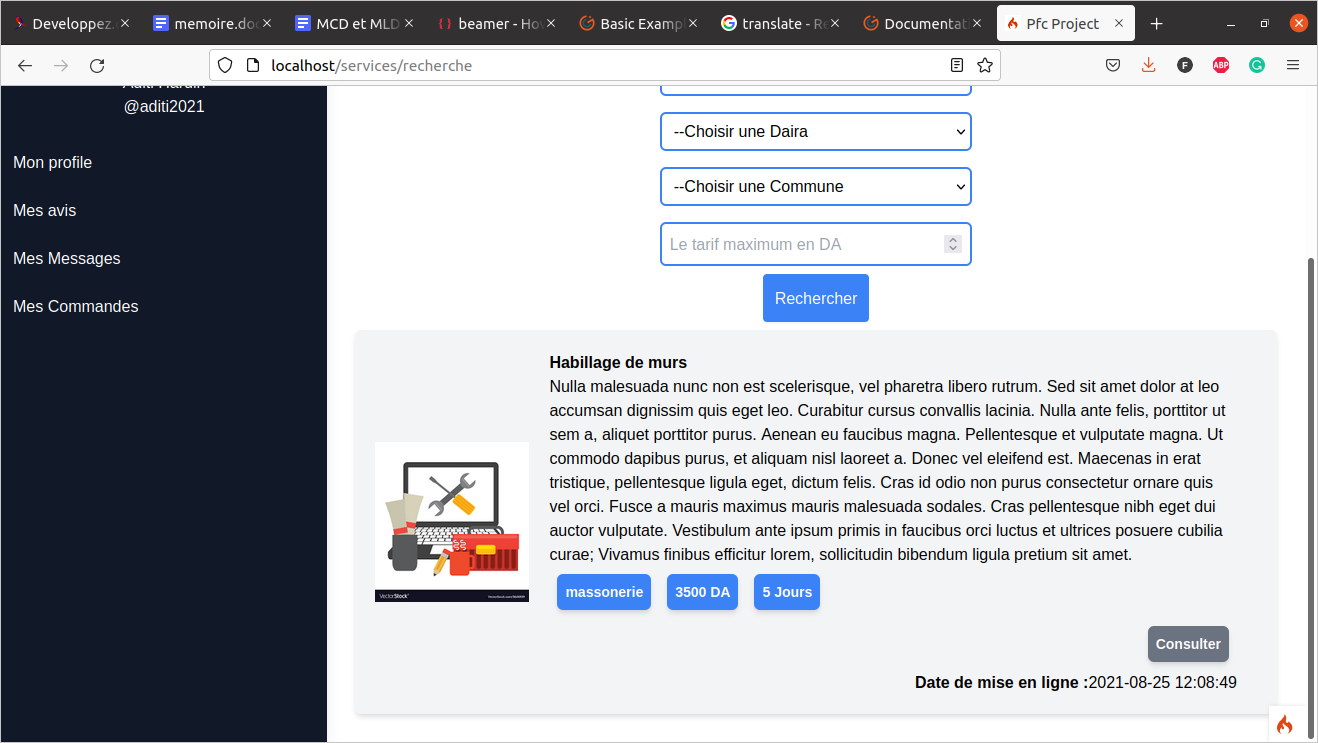
\includegraphics[width=1\textwidth]{images/services.png} 
    \caption{Interface des services}
\end{figure}

Le client pourras consulter le contenu du service (Descriptions, images, tarifs)
et pourras commander le service, contacter le fournisseur et laisser un avis.

 \begin{figure}[H]
    \centering
    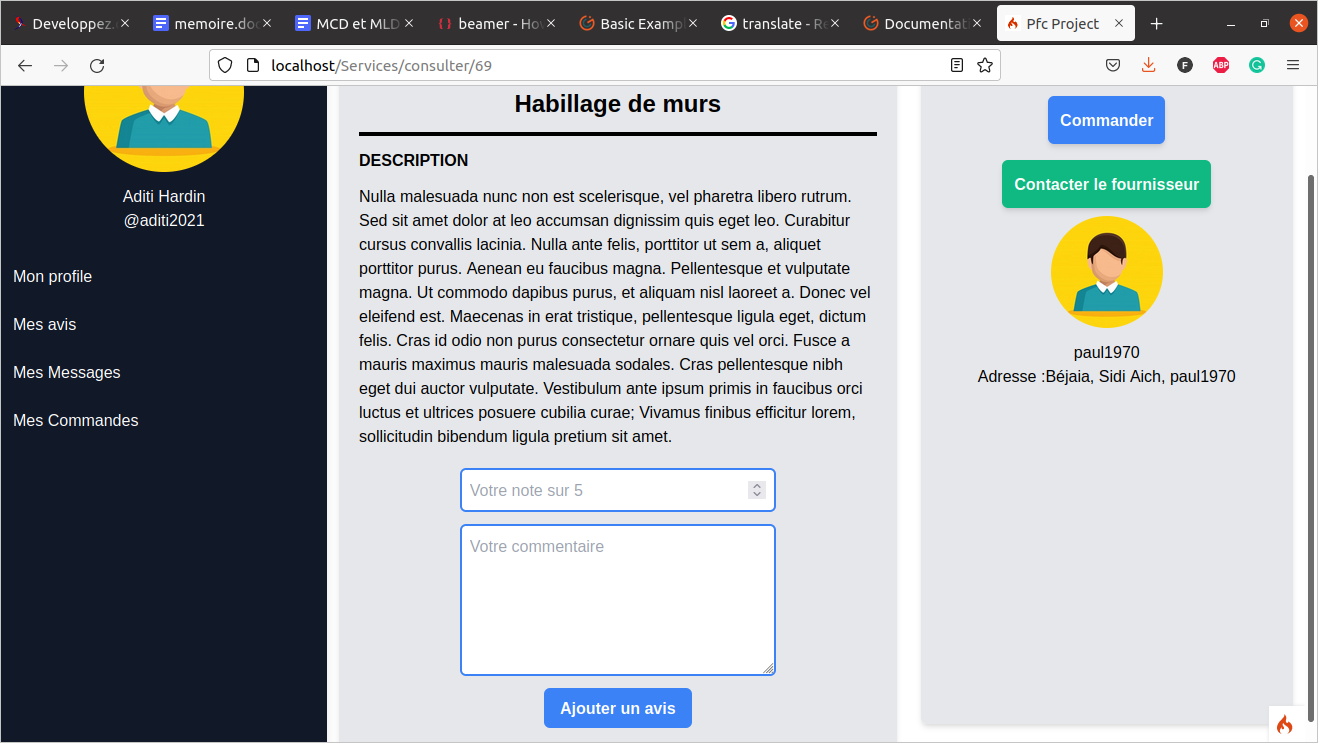
\includegraphics[width=1\textwidth]{images/service consult.png} 
    \caption{Interface des services}
\end{figure}

\subsection{Interface coté fournisseur}

L'interface principale du fournisseur se présente comme suit :

\begin{figure}[H]
    \centering
    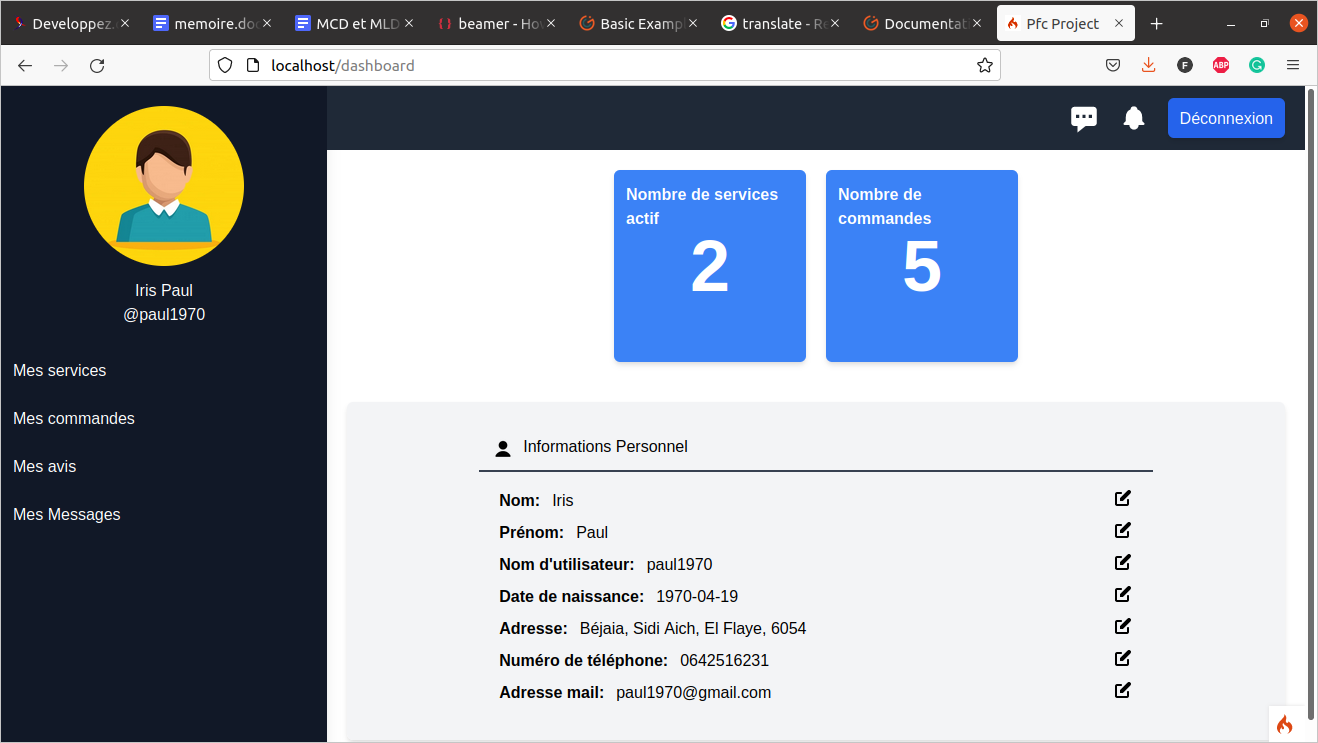
\includegraphics[width=1\textwidth]{images/fourni main.png} 
    \caption{Interface coté Fournisseur}
\end{figure}

Le fournisseur pourras a travers cette interface : 
\begin{itemize}
    \item Voir l'ensemble de ses services et ajouter au besoin
    \item Gérer les commandes reçu
    \item Échanger des messages
    \item Voir quelques statistiques
    
\end{itemize}

\subsection{Conclusion}

Après le chapitre de l'analyse et de la conception, vient la réalisation de
l'application. Dans cette partie technique, nous avons émit les outils et les
environnements utilisé lors de la réalisation, ainsi que les différents langages
de programmation. Puis nous avons citer quelques fonctionnalités de notre
application en s'appuyant sur des capture d'écrans et quelque explication pour
clarifier le fonctionnement des ses fonctionnalités

%Fin du chapitre 3

\section{Conclusion Générale}

Nous sommes parvenus, grâce à ce projet à réaliser une application web sur le
thème ‘ Conception et réalisation d'une application web d'offres de services
professionnel ‘  destinée a tout le monde qui souhait chercher quelqu'un de
qualifier, de professionnel.

Afin d'y parvenir, nous avons débuté notre projet par évoqué la problématique
rencontrer par la plus part des gens lors de leurs recherche de personnes
qualifié offrant leurs services, donner les solutions proposées par notre
application, en précisant ses différentes fonctionnalité, dans le but de mieux
comprendre notre travail. 

Dans le deuxième chapitre, nous évoquons des définitions de l'UML et UP ensuite
nous avons déterminer les différents diagrammes d'UML afin de représenter la
structure globale et l'architecture détaillé de notre système en détaillant son
fonctionnement.

En finissant par un troisième chapitre, où nous avons présenté les différents
outils et langages de développement utilisés pour la réalisation de
l'application, ainsi qu'une présentation de quelques interfaces de celle ci.
    
Dans notre application, nous avons essayé de régler les différents problèmes
que rencontrent les gens au quotidien; (\rmq{non, ce n'est pas vrai.})

\begin{itemize}
    \item Manque d'informations préalables sur une personne.
    \item Manque de moyens pour jauger les compétences d'une personne.
    \item Manque de moyens de contacter directement une personne.
\end{itemize}

\printbibliography

\end{document}
